\part{HTML Elements}

An HTML element is an individual component of an HTML document or "web page", once this has been parsed into the Document Object Model. HTML is composed of a tree of HTML elements and other nodes, such as text nodes. Each element can have HTML attributes specified. Elements can also have content, including other elements and text. HTML elements represent semantics, or meaning. For example, the title element represents the title of the document.

HTML 允许开发者格式化文本,添加图片,创建链接、输入表单、框架和表格等等,并可将之存为文本文件,浏览器即可读取和显示。

HTML 元素指的是从开始标签(start tag)到结束标签(end tag)的所有代码\footnote{开始标签常被称为开放标签(opening tag),结束标签常称为闭合标签(closing tag)。}。元素(elements)用于结构化HTML文档,并告知浏览器如何呈现网页。一般来说,元素由首标签(start tag)、内容(content)和尾标签(end tag)构成,因此HTML 的关键是标签,其作用是指示将出现的内容。




\begin{compactitem}
\item HTML 标签是由尖括号包围的关键词,比如 <html>
\item HTML 标签通常是成对出现的,比如 <b> 和 </b>
\item 标签对中的第一个标签是开始标签,第二个标签是结束标签
\item 开始和结束标签也被称为开放标签和闭合标签
\end{compactitem}




In the HTML syntax, most elements are written with a start tag and an end tag, with the content in between. An HTML tag is composed of the name of the element, surrounded by angle brackets. An end tag also has a slash after the opening angle bracket, to distinguish it from the start tag. For example, a paragraph, which is represented by the p element, would be written as

\begin{lstlisting}[language=HTML]
<p>In the HTML syntax, most elements are written ...</p>
\end{lstlisting}


However, not all of these elements require the end tag, or even the start tag, to be present. Some elements, the so-called void elements, do not have an end tag. A typical example is the br element, which represents a significant line break, such as in a poem or an address. A void element's behaviour is predefined, and it can not contain any content or other elements. For example, the address of the dentist in Finding Nemo would be written as


\begin{lstlisting}[language=HTML]
<p>P. Sherman<br>42 Wallaby Way<br>Sydney</p>
\end{lstlisting}

首标签和尾标签总是必须的吗?

常言道,凡事均有例外。在HTML中,也有例外的情况,即有些元素没有尾标签。这些没有尾标签的元素被称作空元素(empty element),它们与具体文本内容无关,比如像下面这个换行标签:<br />。

大多数浏览器不介意标签是大写还是小写,或者混合大小写。所以<HTML>、<html>或<HtMl>在浏览器上的显示效果都一样。但是,正确的写法是采用小写字母来书写标签。所以,要养成用小写字母书写标签的习惯\footnote{HTML 标签对大小写不敏感:<P> 等同于 <p>,但万维网联盟(W3C)在 HTML 4 中推荐使用小写,而在未来 (X)HTML 版本中强制使用小写。}。

创建HTML文档的过程,也就是在HTML文档里书写标签。一个网站可能包含多个HTML文档。上网的过程,其实就是打开不同HTML文档的过程。

浏览器解析HTML就跟我们读书一样,也是从上往下,从左到右进行的。所以,HTML文档的开始和结束便对应于网页的头和尾。

\begin{compactitem}
\item HTML 文档描述网页
\item HTML 文档包含 HTML 标签和纯文本
\item HTML 文档也被称为网页
\end{compactitem}

When using an XHTML DTD, it is required to open and close the element with a single tag. To specify that it is a void element, a "/" is included at the end of the tag (not to be confused with the "/" at the beginning of a closing tag).

\begin{lstlisting}[language=HTML]
<p>P. Sherman<br/>42 Wallaby Way<br/>Sydney</p>
\end{lstlisting}

标签(tag)指示元素的起始与结束,并且所有标签都具有相同的格式:以小于号“<”开头,以大于号“>”结尾。

一般说来,有两种标签——首标签(start tag)(如<html>)和尾标签(end tag)(如</html>)。它们唯一的区别在于,尾标签多一条斜杠“/。用户通过把内容放在首标签和尾标签之间来对内容进行标记。

HTML主要就是各种各样的元素,所以,学习HTML,就是学习使用各种元素。

\begin{lstlisting}[language=HTML]
<!DOCTYPE html>
<html>
	<head>
		<title>My first HTML.</title>
	</head>
	<body>
	<h1>My first Heading</h1>
	<p>My first paragraph.</p>
	</body>
</html>
\end{lstlisting}

\begin{compactitem}
\item <html> 与 </html> 之间的文本描述网页
\item <head>与</head>之间的文本提供当前网页的信息
\item <title>与</title>之间的文本指定HTML文档的标题
\item <body> 与 </body> 之间的文本是可见的页面内容
\item <h1> 与 </h1> 之间的文本被显示为标题
\item <p> 与 </p> 之间的文本被显示为段落
\end{compactitem}

其中:

\begin{compactitem}
\item <html> 元素定义了整个 HTML 文档。
这个元素拥有一个开始标签 <html>,以及一个结束标签 </html>。
\item <body> 元素定义了 HTML 文档的主体。
这个元素拥有一个开始标签 <body>,以及一个结束标签 </body>。
\item <p> 元素定义了 HTML 文档中的一个段落。
这个元素拥有一个开始标签 <p>,以及一个结束标签 </p>。
\item 即使用户忘记了使用结束标签,大多数浏览器也会正确地显示 HTML\footnote{未来的 HTML 版本不允许省略结束标签。}。
\end{compactitem}

注意,网页标题(title)不是显示在网页里,而是显示在浏览器窗口的标题栏上的。网页里显示的所有内容都必须放在body元素里。

网页标题(title)尤其重要,因为搜索引擎(比如Google)要用它来索引网页,并显示在搜索结果里。

HTML attributes are specified inside the start tag. For example, the abbr element, which represents an abbreviation, expects a title attribute within its opening tag. This would be written as


\begin{lstlisting}[language=HTML]
	<abbr title="abbreviation">abbr.</abbr>
\end{lstlisting}


\chapter{Concepts}


\section{Document vs. DOM}

HTML documents are delivered as "documents". These are then parsed, which turns them into the Document Object Model (DOM) internal representation, within the web browser.

Presentation by the web browser, such as screen rendering or access by JavaScript, is then performed on this internal model, not the original document.

Early HTML documents, and to a lesser extent today, were largely invalid HTML and riddled with syntax errors. The parsing process was also required to "fix-up" these errors, as best it could. The resultant model was often not correct (i.e. it did not represent what a careless coder had originally intended), but it would at least be valid, according to the HTML standard. A valid model was produced, no matter how bad the "tag soup" supplied had been. Only in the rarest cases would the parser abandon parsing altogether.


\section{Elements vs. tags}

"Elements" and "tags" are terms that are widely confused. HTML documents contain tags, but do not contain the elements. The elements are only generated after the parsing step, from these tags.

As is generally understood, the position of an element is indicated as spanning from a start tag, possibly including some child content, and is terminated by an end tag. This is the case for many, but not all, elements within an HTML document.

As HTML is based on SGML, its parsing also depends on the use of a DTD, specifically an HTML DTD such as that for HTML 4.01. The DTD specifies which element types are possible (i.e. it defines the set of element types that go to make up HTML) and it also specifies the valid combinations in which they may appear in a document. It is part of general SGML behaviour that where only one valid structure is possible (per the DTD), it is not generally a requirement that the document explicitly states that structure. As a simple example, the <p> start tag indicating the start of a paragraph element should be closed by a </p> end tag, indicating the end of the element. Also the DTD states that paragraph elements cannot be nested. The HTML document fragment:


\begin{lstlisting}[language=HTML]
<p>Para 1 <p>Para 2 <p>Para 3
\end{lstlisting}

can thus be inferred to be equivalent to:

\begin{lstlisting}[language=HTML]
<p>Para 1 </p><p>Para 2 </p><p>Para 3
\end{lstlisting}

(If one paragraph element cannot contain another, any currently open paragraph must be closed before starting another.)

Because of this implied behaviour, based on the combination of the DTD and the individual document, it is not possible to infer elements from the document tags alone, but only by also using an SGML or HTML aware parser, with knowledge of the DTD.


\section{SGML vs. XML}

SGML is complex, which has limited its widespread adoption and understanding. XML was developed as a simpler alternative. XML is similar to SGML, and can also use the DTD mechanism to specify the elements supported and their permitted combinations as document structure. XML parsing is however simpler. The relation from tags to elements is always simply that of parsing the actual tags included in the document, without the implied closures that are part of SGML.

Where HTML can be formed as XML, either through XHTML or through HTML5 as XML, the parsing from document tags to DOM elements is simplified, but still follows the same basic process. Once the DOM of elements is obtained, behaviour beyond that point (i.e. screen rendering) is identical.


\section{Content vs. Presentation}

Since HTML 4, HTML has increasingly focussed on the separation of content from presentation.[7] This is often referred to as a separation of concerns. HTML is used to represent the structure or content of a document, its presentation remains the sole responsibility of CSS. A default style sheet is suggested as part of the CSS standard, giving a default rendering for HTML.


\section{\%block; vs. box}


Part of this CSS presentation behaviour is the notion of the "box model". This is applied to those elements that CSS considers to be "block" elements, set through the CSS display: block; statement.

HTML also has a similar concept, although different, and the two are very frequently confused. \%block; and \%inline; are groups within the HTML DTD that group elements as being either "block-level" or "inline".[9] This is used to define their nesting behaviour: block-level elements cannot be placed into an inline context.[note 7] This behaviour cannot be changed, it is fixed in the DTD. Block and inline elements have the appropriate and different CSS behaviours attached to them by default,[9] including the relevance of the box model for particular element types.

Note though that this CSS behaviour can, and frequently is, changed from the default. Lists with <ul><li> ... are \%block; elements and are presented as block elements by default. However, it is quite common to set these with CSS to display as an inline list.






\chapter{Overview}

\section{Syntax}


There are multiple kinds of HTML elements: void elements, raw text elements, and normal elements.


\begin{compactenum}
\item Void elements

Void elements only have a start tag, which contains any HTML attributes. They may not contain any children, such as text or other elements. Often they are place holders for elements which reference external files, such as the image (<img/>) element. The attributes included in the element will then point to the external file in question. Another example of a void element is the link element, for which the syntax is

\begin{lstlisting}[language=HTML]
<link rel="stylesheet" href="fancy.css" type="text/css">
\end{lstlisting}

This link element points the browser at a style sheet to use when presenting the HTML document to the user. Note that in the HTML syntax, attributes don't have to be quoted. When using the XML syntax (XHTML), on the other hand, all attributes must be quoted, and a trailing slash is required before the last angle bracket:


\begin{lstlisting}[language=HTML]
<link rel="stylesheet" href="fancy.css" type="text/css" />
\end{lstlisting}


\item Raw text elements

Raw text elements are constructed with:

\begin{compactitem}
\item a start tag (<tag>) marking the beginning of an element, which may incorporate any number of HTML attributes;
\item some amount of text content, but no elements (all tags, apart from the applicable end tag, will be interpreted as content);
\item an end tag, in which the element name is prefixed with a slash: </tag>. In some versions of HTML, the end tag is optional for some elements. The end tag is required in XHTML.
\end{compactitem}

\item Normal elements

Normal elements usually have both a start tag and an end tag, although for some elements the end tag, or both tags, can be omitted. It is constructed in a similar way:

\begin{compactitem}
\item a start tag (<tag>) marking the beginning of an element, which may incorporate any number of HTML attributes;
\item some amount of content, including text and other elements;
\item an end tag, in which the element name is prefixed with a slash: </tag>.
\end{compactitem}

\end{compactenum}


\begin{figure}
\centering
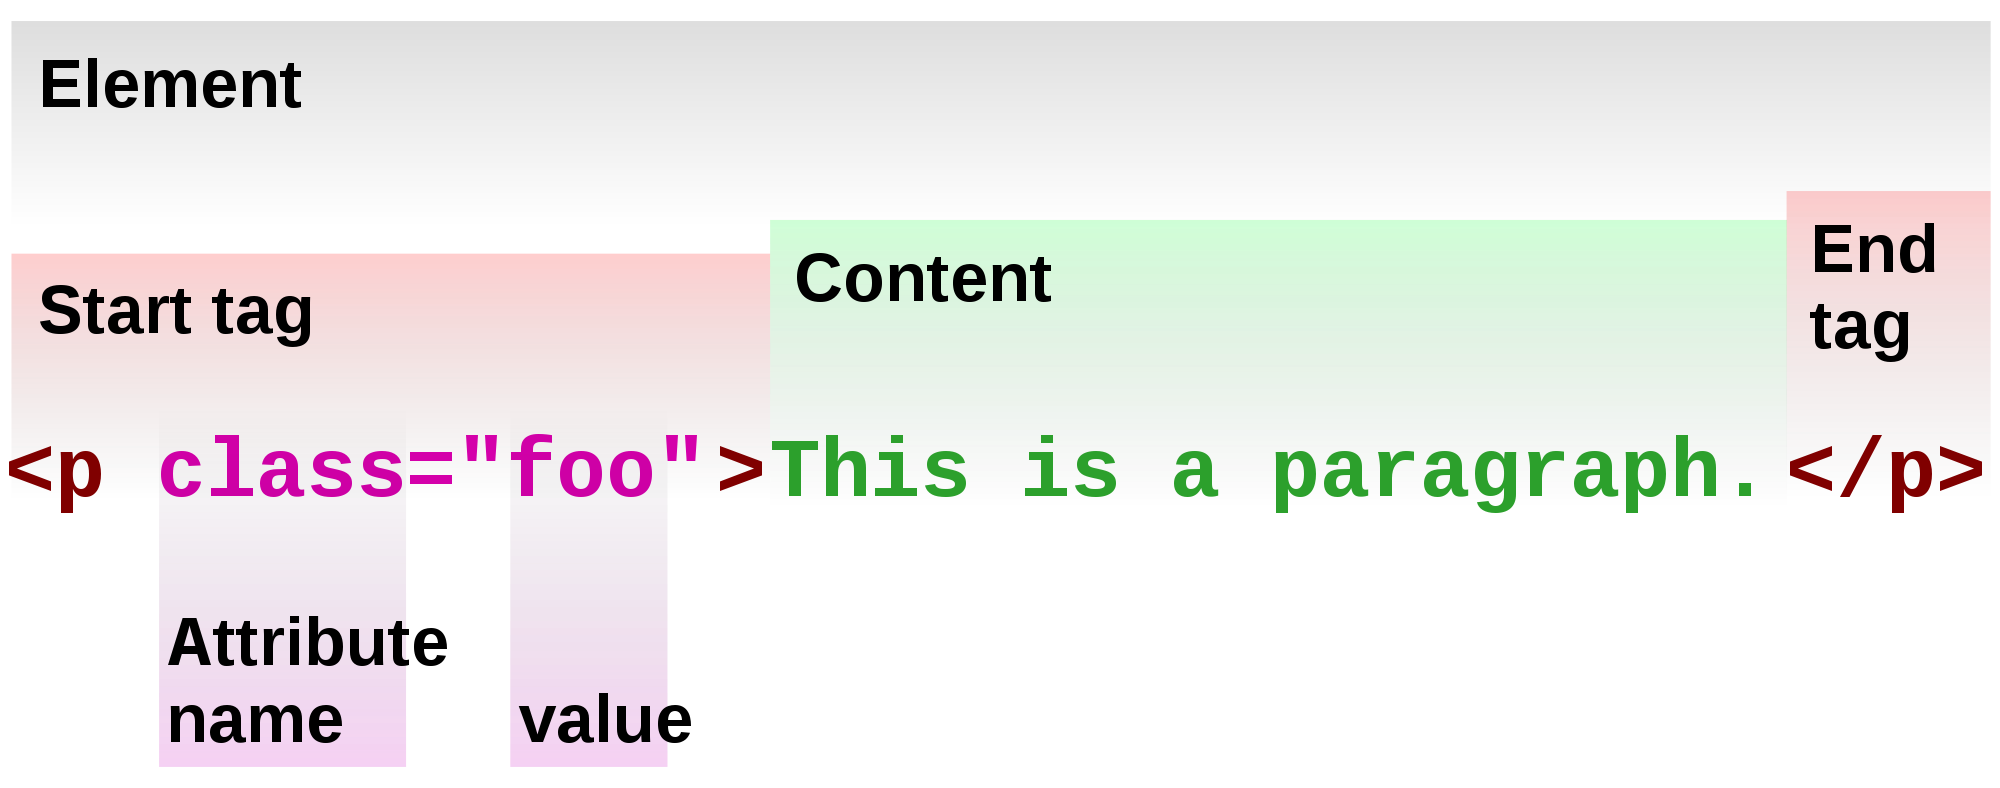
\includegraphics[scale=0.15]{2000px-HTML_element_structure.png}
\caption{Parts of an HTML container element}
\label{HTML_element_structure}
\end{figure}

Parts of an HTML container element:

\begin{compactitem}
\item Start tag: <p ... >
	\begin{compactitem}
	\item Attribute:
		\begin{compactitem}
		\item name: class
		\item value: foo
		\end{compactitem}
	\end{compactitem}
\item Content: This is a paragraph.
\item End tag: </p>
\end{compactitem}



HTML attributes define desired behaviour or indicate additional element properties. Most attributes require a value. In HTML, the value can be left unquoted if it doesn't include spaces (name=value), or it can be quoted with single or double quotes (name='value' or name="value"). In XML, those quotes are required. Boolean attributes, on the other hand, don't require a value to be specified. An example is the checked for checkboxes:



\begin{lstlisting}[language=HTML]
<input type=checkbox checked>
\end{lstlisting}

In the XML syntax, though, the name should be repeated as the value:

\begin{lstlisting}[language=HTML]
<input type="checkbox" checked="checked" />
\end{lstlisting}


Informally, HTML elements are sometimes referred to as "tags" (an example of synecdoche), though many prefer the term tag strictly in reference to the markup delimiting the start and end of an element.

Element (and attribute) names may be written in any combination of upper or lower case in HTML, but must be in lower case in XHTML.[11] The canonical form was upper-case until HTML 4, and was used in HTML specifications, but in recent years, lower-case has become more common.


HTML 元素语法

\begin{compactitem}
\item HTML 元素以开始标签起始
\item HTML 元素以结束标签终止
\item 元素的内容是开始标签与结束标签之间的内容
\item 某些 HTML 元素具有空内容(empty content)
\item 空元素在开始标签中进行关闭(以开始标签的结束而结束)
\item 大多数 HTML 元素可拥有属性
\end{compactitem}

我们无法确定 HTML 被显示的确切效果。屏幕的大小,以及对窗口的调整都可能导致不同的结果。
对于 HTML,用户无法通过在 HTML 代码中添加额外的空格或换行来改变输出的效果。

当显示页面时,浏览器会移除源代码中多余的空格和空行。所有连续的空格或空行都会被算作一个空格。需要注意的是,HTML 代码中的所有连续的空行(换行)也被显示为一个空格。

\section{Elements standards}


HTML elements are defined in a series of freely available open standards issued since 1995, initially by the IETF and subsequently by the W3C.

Since the early 1990s, developers of user agents (e.g. web browsers) have often developed their own elements, some of which have been adopted in later standards. Other user agents may not recognize non-standard elements, and they may be ignored or displayed improperly.

In 1998, XML (a simplified form of SGML) introduced mechanisms to allow anyone to develop their own elements and incorporate them in XHTML documents, for use with XML-aware user agents.

Subsequently, HTML 4.01 was rewritten in an XML-compatible form, XHTML 1.0 (eXtensible HTML). The elements in each are identical, and in most cases valid XHTML 1.0 documents will be valid or nearly valid HTML 4.01 documents. This article mainly focuses on real HTML, unless noted otherwise; however, it remains applicable to XHTML. (See HTML for a discussion of the minor differences between the two).


\section{Elements status}


Since the first version of HTML, several elements have become outmoded, and are deprecated in later standards, or do not appear at all, in which case they are invalid (and will be found invalid, and perhaps not displayed, by validating user agents).

At present, the status of elements is complicated by the existence of three types of HTML 4.01 / XHTML 1.0 DTD:

\begin{compactitem}
\item Transitional, which contain deprecated elements, but which were intended to provide a transitional period during which authors could update their practices;
\item Frameset, which are versions of the Transitional DTDs which also allow authors to write frameset documents;
\item Strict, which is the up-to date (as at 1999) form of HTML.
\end{compactitem}

The first Standard (HTML 2.0) contained four deprecated elements, one of which was invalid in HTML 3.2. All four are invalid in HTML 4.01 Transitional, which also deprecated a further ten elements. All of these, plus two others, are invalid in HTML 4.01 Strict. While the frame elements are still current in the sense of being present in the Transitional and Frameset DTDs, there are no plans to preserve them in future standards, as their function has been largely replaced, and they are highly problematic for user accessibility.


(Strictly speaking, the most recent XHTML standard, XHTML 1.1 (2001), does not include frames at all; it is approximately equivalent to XHTML 1.0 Strict, but also includes the Ruby markup module.)

A common source of confusion is the loose use of deprecated to refer to both deprecated and invalid status, and to elements which are expected to be formally deprecated in future.

\section{Presentation and behaviour}





In keeping with the principle of separation of concerns, the function of HTML is primarily to add structural and semantic information to the raw text of a document. Presentation and behaviour are separate functions, which can be added as desired, ideally through links to external documents such as style sheets, graphics files, and scripts.

This allows the document to be presented by different user agents according to their purposes and abilities; for example, a user agent can select an appropriate style sheet to present a document by displaying on a monitor, printing on paper, or to determine speech characteristics in an aural user agent. The structural and semantic functions of the markup remain identical in each case.

Historically, user agents did not always support these features. In the 1990s, as a stop-gap, presentational elements were added to HTML, at the cost of creating problems for interoperability and user accessibility. This is now regarded as outmoded and has been superseded by style sheet-based design; most presentational elements are now deprecated.

External image files are incorporated with the img or object elements. (With XHTML, the SVG language can also be used to write graphics within the document, though linking to external SVG files is generally simpler.) Where an image is not purely decorative, HTML allows replacement content with similar semantic value to be provided for non-visual user agents.


An HTML document can also be extended through the use of scripts to provide additional behaviours beyond the abilities of HTML hyperlinks and forms.

The elements style and script, with related HTML attributes, provide reference points in HTML markup for links to style sheets and scripts. They can also contain instructions directly.

\begin{compactitem}
\item In the document head, script and style may either link to shared external documents, or contain embedded instructions. (The link element can also be used to link style sheets.)
\item The style attribute is valid in most document body elements for inclusion of inline style instructions.
\item Event-handling attributes, which provide links to scripts, are optional in most elements.
script can occur at any point in the document body.
\item For user agents which do not operate scripts, the noscript element provides alternative content where appropriate; however, it can only be used as a block-level element.
\end{compactitem}


\section{List of all HTML4.01/XHTML1.0 elements}

DTD:指示在哪种 XHTML 1.0 DTD 中允许该标签。S=Strict, T=Transitional, F=Frameset。



\begin{longtable}{|p{60pt}|p{320pt}|p{40pt}|}
\multicolumn{3}{r}{...}
\tabularnewline\hline
Tag				& Description		& DTD		
\endhead
\hline
Tag				& Description		& DTD	
\tabularnewline\hline
\endfirsthead
\multicolumn{3}{r}{...}
\endfoot
%\tabularnewline\hline
\endlastfoot
<!--...-->		&	Defines a comment			& STF	\\
\hline
<!DOCTYPE>	&	Defines the document type	& STF	\\
\hline
<a>			&	Defines a hyperlink			& STF	\\
\hline
<abbr>		&	Defines an abbreviation		& STF	\\
\hline
<acronym>	&	Not supported in HTML5. Defines an acronym	& STF	\\
\hline
<address>	&	Defines contact information for the author/owner of a document & STF\\
\hline
<applet>		&	Not supported in HTML5. Deprecated in HTML 4.01. Defines an embedded applet	& TF	\\
\hline
<area>		&	Defines an area inside an image-map & STF\\
\hline
<article>		&	Defines an article & STF\\
\hline
<aside>		&	Defines content aside from the page content & STF\\
\hline
<audio>		&	Defines sound content & STF\\
\hline
<b>			&	Defines bold text & STF\\
\hline
<base>		&	Specifies the base URL/target for all relative URLs in a document & STF\\
\hline
<basefont>	&	Not supported in HTML5. Deprecated in HTML 4.01. Specifies a default colour, size, and font for all text in a document & TF\\
\hline
<bdi>		&	Isolates a part of text that might be formatted in a different direction from other text outside it & STF\\
\hline
<bdo>		&	Overrides the current text direction & STF\\
\hline
<big>		&	Not supported in HTML5. Defines big text & STF\\
\hline
<blockquote>	&	Defines a section that is quoted from another source & STF\\
\hline
<body>		&	Defines the document's body & STF\\
\hline
<br>			&	Defines a single line break	& STF\\
\hline
<canvas>		&	Used to draw graphics, on the fly, via scripting (usually JavaScript) & STF\\
\hline
<caption>		&	Defines a table caption & STF\\
\hline
<center>		&	Not supported in HTML5. Deprecated in HTML 4.01. Defines centred text & TF\\
\hline
<cite>		&	Defines the title of a work & STF\\
\hline
<code>		&	Defines a piece of computer code & STF\\
\hline
<col>		&	Specifies column properties for each column within a <colgroup> element  & STF\\
\hline
<colgroup>	&	Specifies a group of one or more columns in a table for formatting	& STF\\
\hline
<command>	&	Defines a command button that a user can invoke	& STF\\
\hline
<datalist>	&	Specifies a list of pre-defined options for input controls & STF\\
\hline
<dd>		&	Defines a description of an item in a definition list & STF\\
\hline
<del>		&	Defines text that has been deleted from a document & STF\\
\hline
<details>		&	Defines additional details that the user can view or hide & STF\\
\hline
<dfn>		&	Defines a definition term & STF\\
\hline
<dialog>		&	Defines a dialog box or window & STF\\
\hline
<dir>		&	Not supported in HTML5. Deprecated in HTML 4.01. Defines a directory list & TF\\
\hline
<div>		&	Defines a section in a document	& STF\\
\hline
<dl>			&	Defines a definition list & STF\\
\hline
<dt>			&	Defines a term (an item) in a definition list & STF\\
\hline
<em>		&	Defines emphasized text & STF\\
\hline
<embed>		&	Defines a container for an external (non-HTML) application & STF\\
\hline
<fieldset>	&	Groups related elements in a form	& STF\\
\hline
<figcaption>	&	Defines a caption for a <figure> element & STF\\
\hline
<figure>		&	Specifies self-contained content & STF\\
\hline
<font>		&	Not supported in HTML5. Deprecated in HTML 4.01. Defines font, colour, and size for text & TF\\
\hline
<footer>		&	Defines a footer for a document or section & STF\\
\hline
<form>		&	Defines an HTML form for user input & STF\\
\hline
<frame>		&	Not supported in HTML5. Defines a window (a frame) in a frameset & F \\
\hline
<frameset>	&	Not supported in HTML5. Defines a set of frames & F\\
\hline
<h1> to <h6>	&	Defines HTML headings & STF\\
\hline
<head>		&	Defines information about the document & STF\\
\hline
<header>		&	Defines a header for a document or section & STF\\
\hline
<hgroup>		&	Groups heading (<h1> to <h6>) elements & STF\\
\hline
<hr>			&	Defines a thematic change in the content & STF\\
\hline
<html>		&	Defines the root of an HTML document & STF\\
\hline
<i>			&	Defines a part of text in an alternate voice or mood & STF\\
\hline
<iframe>		&	Defines an inline frame & TF\\
\hline
<img>		&	Defines an image & STF\\
\hline
<input>		&	Defines an input control & STF\\
\hline
<ins>		&	Defines a text that has been inserted into a document & STF\\
\hline
<kbd>		&	Defines keyboard input & STF\\
\hline
<keygen>		&	Defines a key-pair generator field (for forms) & STF\\
\hline
<label>		&	Defines a label for an <input> element & STF\\
\hline
<legend>		&	Defines a caption for a <fieldset>, < figure>, or <details> element & STF\\
\hline
<li>			&	Defines a list item & STF\\
\hline
<link>		&	Defines the relationship between a document and an external resource (most used to link to style sheets)	 & STF\\
\hline
<map>		&	Defines a client-side image-map & STF\\
\hline
<mark>		&	Defines marked/highlighted text & STF\\
\hline
<menu>		&	Defines a list/menu of commands &TF\\
\hline
<meta>		&	Defines metadata about an HTML document & STF\\
\hline
<meter>		&	Defines a scalar measurement within a known range (a gauge) & STF\\
\hline
<nav>		&	Defines navigation links & STF\\
\hline
<noframes>	&	Not supported in HTML5. Defines an alternate content for users that do not support frames & TF\\
\hline
<noscript>	&	Defines an alternate content for users that do not support client-side scripts & STF\\
\hline
<object>		&	Defines an embedded object & STF\\
\hline
<ol>			&	Defines an ordered list & STF\\
\hline
<optgroup>	&	Defines a group of related options in a drop-down list & STF\\
\hline
<option>		&	Defines an option in a drop-down list & STF\\
\hline
<output>		&	Defines the result of a calculation & STF\\
\hline
<p>			&	Defines a paragraph & STF\\
\hline
<param>		&	Defines a parameter for an object & STF\\
\hline
<pre>		&	Defines pre-formatted/space-preserving text & STF\\
\hline
<progress>	&	Represents the progress of a task & STF\\
\hline
<q>			&	Defines a short quotation & STF\\
\hline
<rp>			&	Defines what to show in browsers that do not support ruby annotations & STF\\
\hline
<rt>			&	Defines an explanation/pronunciation of characters (for East Asian typography) & STF\\
\hline
<ruby>		&	Defines a ruby annotation (for East Asian typography) & STF\\
\hline
<s>			&	Defines text that is no longer correct	& TF\\
\hline
<samp>		&	Defines sample output from a computer program & STF\\
\hline
<script>		&	Defines a client-side script & STF\\
\hline
<section>		&	Defines a section in a document & STF\\
\hline
<select>		&	Defines a drop-down list & STF\\
\hline
<small>		&	Defines smaller text & STF\\
\hline
<source>		&	Defines multiple media resources for media elements (<video> and <audio>) & STF\\
\hline
<span>		&	Defines a section in a document & STF\\
\hline
<strike>		&	Not supported in HTML5. Deprecated in HTML 4.01. Defines strike-through text & TF\\
\hline
<strong>		&	Defines important text & STF\\
\hline
<style>		&	Defines style information for a document & STF \\
\hline
<sub>		&	Defines subscripted text & STF\\
\hline
<summary>	&	Defines a visible heading for a <details> element & STF\\
\hline
<sup>		&	Defines superscripted text & STF\\
\hline
<table>		&	Defines a table & STF\\
\hline
<tbody>		&	Groups the body content in a table & STF\\
\hline
<td>			&	Defines a cell in a table & STF\\
\hline
<textarea>	&	Defines a multi-line input control (text area) & STF\\
\hline
<tfoot>		&	Groups the footer content in a table & STF\\
\hline
<th>			&	Defines a header cell in a table & STF\\
\hline
<thead>		&	Groups the header content in a table & STF\\
\hline
<time>		&	Defines a date/time & STF\\
\hline
<title>		&	Defines a title for the document & STF\\
\hline
<tr>			&	Defines a row in a table & STF\\
\hline
<track>		&	Defines text tracks for media elements (<video> and <audio>) & STF\\
\hline
<tt>			&	Not supported in HTML5. Defines Teletype text & STF\\
\hline
<u>			&	Defines text that should be stylistically different from normal text & TF\\
\hline
<ul>			&	Defines an unordered list & STF\\
\hline
<var>		&	Defines a variable & STF\\
\hline
<video>		&	Defines a video or movie & STF\\
\hline
<wbr>		&	Defines a possible line-break & STF\\
\hline
\end{longtable}



\chapter{Document structure elements}


\section{<html>...</html>}

The Root element of an HTML document; all other elements are contained in this.

The HTML element delimits the beginning and the end of an HTML document.

Standardized in HTML 2.0; still current.


\section{<head>...</head>}

Container for processing information and metadata for an HTML document.

Standardized in HTML 2.0; still current.

<head> 元素是所有头部元素的容器。<head> 内的元素可包含脚本,指示浏览器在何处可以找到样式表,提供元信息,等等。

以下标签都可以添加到 head 部分:<title>、<base>、<link>、<meta>、<script> 以及 <style>。

\subsection{<title>...</title>}

<title> 标签定义文档的标题。

title 元素在所有 HTML/XHTML 文档中都是必需的,title 元素能够:

\begin{compactitem}
\item 定义浏览器工具栏中的标题
\item 提供页面被添加到收藏夹时显示的标题
\item 显示在搜索引擎结果中的页面标题
\end{compactitem}

一个简化的 HTML 文档代码如下:

\begin{lstlisting}[language=HTML]
<!DOCTYPE html>
<html>
  <head>
    <title>Title of the document</title>
  </head>
  <body>
    The content of the document......
  </body>
</html>
\end{lstlisting}

\subsection{<base>...</base>}

<base> 标签为页面上的所有链接规定默认地址或默认目标(target):

\begin{lstlisting}[language=HTML]
<head>
  <base href="URL/contents/" />
  <base target="_blank" />
</head>
\end{lstlisting}


\subsection{<link>...</link>}

<link> 标签定义文档与外部资源之间的关系,<link> 标签最常用于连接样式表:

\begin{lstlisting}[language=HTML]
    <head>
      <link rel="stylesheet" type="text/css" href="style.css" />
    </head>
\end{lstlisting}

\subsection{<style>...</style>}

<style> 标签用于为 HTML 文档定义样式信息,可以在 style 元素内规定 HTML 元素在浏览器中呈现的样式:

\begin{lstlisting}[language=HTML]
<head>
  <style type="text/css">
    body {background-color:yellow}
    p {color:blue}
  </style>
</head>
\end{lstlisting}


\subsection{<meta>...</meta>}

元数据(metadata)是关于数据的信息。

<meta> 标签提供关于 HTML 文档的元数据。元数据不会显示在页面上,但是对于机器是可读的。

典型的情况是,meta 元素被用于规定页面的描述、关键词、文档的作者、最后修改时间以及其他元数据。

<meta> 标签始终位于 head 元素中。

元数据可用于浏览器(如何显示内容或重新加载页面),搜索引擎(关键词),或其他 web 服务。


一些搜索引擎会利用 meta 元素的 name 和 content 属性来索引您的页面。

下面的 meta 元素定义页面的描述:

\begin{lstlisting}[language=HTML]
  <meta name="description" content="Free Web tutorials on HTML, CSS, XML" />
\end{lstlisting}


下面的 meta 元素定义页面的关键词:

\begin{lstlisting}[language=HTML]
  <meta name="keywords" content="HTML, CSS, XML" />
\end{lstlisting}

name 和 content 属性的作用是描述页面的内容。

下面的meta元素定义把用户重定向到新的网址,打开网页5秒之后,用户将被重定向到URL所指示的新页面。

\begin{lstlisting}[language=HTML]
  <meta http-equiv="Refresh" content="5;url=URL" />
\end{lstlisting}


\subsection{<script>...</script>}

<script> 标签用于定义客户端脚本,比如 JavaScript,JavaScript可以使 HTML 页面具有更强的动态和交互性,具体用于图片操作、表单验证以及内容动态更新。

script 元素既可包含脚本语句,也可通过 src 属性指向外部脚本文件,通过必需的 type 属性来规定脚本的 MIME 类型。


\begin{lstlisting}[language=HTML]
  <script type="text/javascript" src="js/jquery.js"></script>
\end{lstlisting}

下面的脚本会向浏览器输出“Hello World!”:

\begin{lstlisting}[language=HTML]
  <script type="text/javascript">
    document.write("Hello World!")
  </script>
\end{lstlisting}

\subsection{<noscript>...</noscript>}

<noscript> 标签提供无法使用脚本时的替代内容,比方在浏览器禁用脚本时,或浏览器不支持客户端脚本时。

noscript 元素可包含普通 HTML 页面的 body 元素中能够找到的所有元素。

只有在浏览器不支持脚本或者禁用脚本时,才会显示 noscript 元素中的内容:

\begin{lstlisting}[language=HTML]
  <script type="text/javascript">
    document.write("Hello World!")
  </script>
  <noscript>Current browser does not support JavaScript!</noscript>
\end{lstlisting}

如果浏览器压根没法识别 <script> 标签,那么 <script> 标签所包含的内容将以文本方式显示在页面上。为了避免这种情况发生,用户应该将脚本隐藏在注释标签当中,于是那些老的浏览器(无法识别 <script> 标签的浏览器)将忽略这些注释,所以不会将标签的内容显示到页面上。而那些新的浏览器将读懂这些脚本并执行它们,即使代码被嵌套在注释标签内。

\begin{lstlisting}[language=HTML]
  Javascript:
  <script type="text/javascript">
    <!--
    document.write("Hello World!")
    //-->
  </script>
  VBScript:
  <script type="text/vbscript">
  <!--
  document.write("Hello World!")
  '-->
  </script>
\end{lstlisting}


\begin{table}[!h]
\centering
\caption{HTML脚本标签}
\begin{tabular}{|l|l|}
\hline
标签			&描述\\
\hline
<script>		&定义客户端脚本。\\
\hline
<noscript>	&为不支持客户端脚本的浏览器定义替代内容。\\
\hline
\end{tabular}
\end{table}


\begin{table}[!h]
\centering
\caption{HTML 头部元素}
\begin{tabular}{|l|l|}
\hline
标签		&描述\\
\hline
<head>	&定义关于文档的信息。\\
\hline
<title>	&定义文档标题。\\
\hline
<base>	&定义页面上所有链接的默认地址或默认目标。\\
\hline
<link>	&定义文档与外部资源之间的关系。\\
\hline
<meta>	&定义关于 HTML 文档的元数据。\\
\hline
<script>	&定义客户端脚本。\\
\hline
<style>	&定义文档的样式信息。\\
\hline
\end{tabular}
\end{table}


\section{<body>...</body>}


Container for the displayable content of an HTML document.

Standardized in HTML 2.0; still current.

<body> 拥有两个配置背景的标签,背景可以是颜色或者图像。

背景颜色属性(bgcolor)将背景设置为某种颜色。属性值可以是十六进制数、RGB 值或颜色名。

\begin{lstlisting}[language=HTML]
	<body bgcolor="#000000">
	<body bgcolor="rgb(0,0,0)">
	<body bgcolor="black">
\end{lstlisting}

以上的代码均将背景颜色设置为黑色。

背景属性(background)将背景设置为图像。属性值为图像的URL。如果图像尺寸小于浏览器窗口,那么图像将在整个浏览器窗口进行复制。

\begin{lstlisting}[language=HTML]
	<body background="bg.gif">
	<body background="URL/bg.gif">
\end{lstlisting}

URL可以是相对地址,如第一行代码。也可以使绝对地址,如第二行代码。

如果用户打算使用背景图片,需要谨记一下几点:
\begin{compactitem}
\item 背景图像是否增加了页面的加载时间,图像文件不应超过 10k。
\item 背景图像是否与页面中的其他图象搭配良好。
\item 背景图像是否与页面中的文字颜色搭配良好。
\item 图像在页面中平铺后,看上去还可以吗?
\item 对文字的注意力被背景图像喧宾夺主了吗?
\end{compactitem}

<body> 标签中的背景颜色(bgcolor)、背景(background)和文本(text)属性在最新的 HTML 标准(HTML4 和 XHTML)中已被废弃。W3C 在他们的推荐标准中已删除这些属性,现在都是使用层叠样式表(CSS)来定义 HTML 元素的布局和显示属性。

\chapter{Document head elements}



\section{<base>}



Specifies a base URL for all relative href and other links in the document. Must appear before any element that refers to an external resource. HTML permits only one base element for each document. The base element has HTML attributes, but no contents.

A development version of BASE is mentioned in HTML Tags; standardized in HTML 2.0; still current.



\pdfstringdefDisableCommands{%
  \let\sout\relax
}

\section{\sout{<basefont>}}

(deprecated)

Specifies a base font size, typeface, and colour for the document. Used together with font elements. Deprecated in favour of style sheets.

Standardized in HTML 3.2; deprecated in HTML 4.0 Transitional; invalid in HTML 4.0 Strict.



\section{\sout{<isindex>}}

(deprecated)

isindex could either appear in the document head or in the body, but only once in a document. 


\section{<link>}

Specifies links to other documents, such as previous and next links, or alternate versions. A common use is to link to external style sheets, using the form:

\begin{lstlisting}[language=HTML]
<link rel="stylesheet" type="text/css" href="url" title="description_of_style">
\end{lstlisting}

A less-common, but important, usage is to supply navigation hints consistently through use of microformats. Several common relationships are defined, that may be exposed to users through the browser interface rather than directly in the web page.

\begin{lstlisting}[language=HTML]
<link rel="next" href="url">
\end{lstlisting}

A document's head element may contain any number of link elements. The link element has HTML attributes, but no contents.

LINK existed in HTML Internet Draft 1.2, and was standardized in HTML 2.0; still current.




\section{<meta>}

<meta> can be used to specify additional metadata about a document, such as its author, publication date, expiration date, page description, keywords, or other information not provided through the other header elements and HTML attributes. Because of their generic nature, meta elements specify associative key-value pairs. In general, a meta element conveys hidden information about the document. Several meta tags can be used, all of which should be nested in the head element. The specific purpose of each meta element is defined by its attributes.

In one form, meta elements can specify HTTP headers which should be sent by a web server before the actual content, for example:

\begin{lstlisting}[language=HTML]
<meta http-equiv="foo" content="bar">
\end{lstlisting}

this specifies that the page should be served with an HTTP header called foo that has a value bar.

In the general form, a meta element specifies name and associated content HTML attributes describing aspects of the HTML page. To prevent possible ambiguity, an optional third attribute, scheme, may be supplied to specify a semantic framework that defines the meaning of the key and its value, for example:

\begin{lstlisting}[language=HTML]
<meta name="foo" content="bar" scheme="DC">
\end{lstlisting}

In this example, the meta element identifies itself as containing the foo element, with a value of bar, from the DC or Dublin Core resource description framework.

Standardized in HTML 2.0; still current.


\section{<object>...</object>}


<object>...</object> can be used for including generic objects within the document header. Though rarely used within a head element, it could potentially be used to extract foreign data and associate it with the current document.

Standardized in HTML 4.0; still current.



\section{<script>...</script>}

<script>...</script> can act as a container for script instructions or link to an external script with the optional src attribute.[20] Also usable in the document body to dynamically generate either both block or inline content.

Standardized in HTML 3.2; still current.



\section{<style>...</style>}

<style>...</style> specifies a style for the document, usually in the form:

\begin{lstlisting}[language=HTML]
  <style type="text/css"> ... </style>
\end{lstlisting}

<style>...</style> can either act as a container for style instructions or link to external style sheets – for example, in CSS, with @import directives of the form:

\begin{lstlisting}[language=HTML]
  <style> @import url; </style>
\end{lstlisting}


Standardized in HTML 3.2; still current.

\section{<title>...</title>}

<title>...</title> define a document title. Required in every HTML and XHTML document. User agents may use the title in different ways. For example:

\begin{compactitem}
\item Web browsers usually display it in a window's title bar when the window is open, and (where applicable) in the task bar when the window is minimized.
\item It may become the default file-name when saving the page.
\item Search engines’ web crawlers may pay particular attention to the words used in the title.
\end{compactitem}

The title element must not contain other elements, only text. Only one title element is permitted in a document.

TITLE existed in HTML Tags, and was standardized in HTML 2.0; still current.




\chapter{Document body elements}


In visual browsers, displayable elements can be rendered as either block or inline. While all elements are part of the document sequence, block elements appear within their parent elements:

\begin{compactitem}
\item as rectangular objects which do not break across lines;
\item with block margins, width and height properties which can be set independently of the surrounding elements.
\end{compactitem}

Conversely, inline elements are treated as part of the flow of document text; they cannot have margins, width or height set, and do break across lines.


\section{Block elements}

Block elements, or block-level elements, have a rectangular structure. By default, these elements will span the entire width of its parent element, and will thus not allow any other element to occupy the same horizontal space as it is placed on.

大多数 HTML 元素被定义为块级元素或内联元素。“块级元素”译为 block level element,“内联元素”译为 inline element。

块级元素在浏览器显示时,通常会以新行来开始(和结束),例如:<h1>, <p>, <ul>, <table>



The rectangular structure of a block element is often referred to as the box model, and is made up of several parts. Each element contains the following:

\begin{compactitem}
\item The content of an element is the actual text (or other media) placed between the opening and closing tags of an element.
\item The padding of an element is the space around that content, which still form part of said element. Padding is physically part of an element, and should not be used to create white space between two elements. Any background style assigned to the element, such as a background image or color, will be visible within the padding. 
\item Increasing the size of an element's padding increases the space this element will take up.
\item The border of an element is the absolute end of an element, and spans the circumference of that element. \item The thickness of a border increases the size of an element.
\item The margin of an element is the white-space that surrounds an element. The content, padding and border of any other element will not be allowed to enter this area, unless forced to do so by some advanced CSS placement. Using most standard DTDs, margins on the left and right of different elements will push each other away. Margins on the top or bottom of an element, on the other hand, will not stack, or will inter mingle. This means that the white-space between these elements will be as big as the larger margin between them.
\end{compactitem}

The above section refers only to the detailed implementation of CSS rendering and has no relevance to HTML elements themselves.



\subsection{Basic text}



\subsubsection{<p>...</p>}

Creates a paragraph, perhaps the most common block\footnote{注释:浏览器会自动地在段落的前后添加空行,因为<p> 是块级元素。} level element.

P existed in HTML Tags, and was standardized in HTML 2.0; still current.

HTML 段落是通过 <p> 标签进行定义的,从而可以把 HTML 文档分割为若干段落\footnote{提示:使用空的段落标记 <p></p> 去插入一个空行是个坏习惯。用 <br /> 标签代替它,但是不要用 <br /> 标签去创建列表。}。





即使忘了使用结束标签,大多数浏览器也会正确地将 HTML 显示出来,但是在未来的 HTML 版本中,不允许省略结束标签\footnote{提示:通过结束标签来关闭 HTML 是一种经得起未来考验的 HTML 编写方法。清楚地标记某个元素在何处开始,并在何处结束,不论对开发者还是对浏览器来说,都会使代码更容易理解。}。






\subsubsection{<h1>...</h1> <h2>...</h2> <h3>...</h3> <h4>...</h4> <h5>...</h5> <h6>...</h6>}

Section headings at different levels. <h1> delimits the highest-level heading, <h2> the next level down (sub-section), <h3> for a level below that, and so on to <h6>. They are sometimes referred to collectively as <hn> tags, n meaning any of the available heading levels.

Most visual browsers show headings as large bold text by default, though this can be overridden with CSS. Heading elements are not intended merely for creating large or bold text—in fact, they should not be used for explicitly styling text. Rather, they describe the document’s structure and organization. Some programs use them to generate outlines and tables of contents.

Headings existed in HTML Tags, and were standardized in HTML 2.0; still current.

在 HTML 文档中,标题很重要。HTML 标题(Heading)是通过 <h1> - <h6> 等标签进行定义的,其中<h1> 定义最大的标题。<h6> 定义最小的标题\footnote{请仅仅把标题标签用于标题文本。不要仅仅为了产生粗体文本而使用它们。}。

注释:浏览器会自动地在标题的前后添加空行。

注释:默认情况下,HTML 会自动地在块级元素前后添加一个额外的空行,比如段落、标题元素前后。

\begin{compactitem}
\item 确保将 HTML heading 标签只用于标题。不要仅仅是为了产生粗体或大号的文本而使用标题。
\item 搜索引擎使用标题为网页的结构和内容编制索引。
\item 因为用户可以通过标题来快速浏览网页,所以用标题来呈现文档结构是很重要的。
\item 应该将 h1 用作主标题(最重要的),其后是 h2(次重要的),再其次是 h3,以此类推。
\end{compactitem}

\subsection{List}


\subsubsection{<dl>...</dl>}

An association list consisting of name-value groups (previously to HTML5 defined as a definition list; consisting of definition terms paired with definitions).

自定义列表不仅仅是一列项目,而是项目及其注释的组合。

自定义列表以 <dl> 标签开始。每个自定义列表项以 <dt> 开始。每个自定义列表项的定义以 <dd> 开始。

\begin{lstlisting}[language=HTML]
	<dl>
		<dt>Coffee</dt>
			<dd>Black hot drink</dd>
		<dt>Milk</dt>
			<dd>White cold drink</dd>
	</dl>
\end{lstlisting}

定义列表的列表项内部可以使用段落、换行符、图片、链接以及其他列表等等。

DL existed in HTML Tags, and was standardized in HTML 2.0; still current.



\subsubsection{<dt>...</dt>}


A name in an association list (previously definition term in a definition list).

DT existed in HTML Tags, and was standardized in HTML 2.0; still current.




\subsubsection{<dd>...</dd>}

The value in an association list (previously definition of a term, in a definition list).

DD existed in HTML Tags, and was standardized in HTML 2.0; still current.






\subsubsection{<ol>...</ol>}


An ordered (enumerated) list. The type attribute can be used to specify the kind of ordering, but style sheets give more control: \{list-style-type: foo\}. The default is Arabic numbering.

有序列表也是一列项目,列表项目使用数字进行标记。有序列表始于 <ol> 标签。每个列表项始于 <li> 标签。

\begin{lstlisting}[language=HTML]
	<ol>
		<li>Coffee</li>
		<li>Milk</li>
	</ol>
\end{lstlisting}

列表项内部可以使用段落、换行符、图片、链接以及其他列表等等。


OL existed in HTML Internet Draft 1.2, and was standardized in HTML 2.0; still current.

Write TYPE=?,replacing ? with the below code for corresponding numbering style code: 'Á'for A,B,C...,'a' for a,b,c...,| for |,||,|||,....i for i,ii,iii(i.e. roman),1 for 1,2,3(decimal).








\subsubsection{<ul>...</ul>}

An unordered (bulleted) list. Style sheets can be used to specify the list marker: \{list-style-type: foo\}. The default marker is a disc.

无序列表是一个项目的列表,此列项目使用粗体圆点(典型的小黑圆圈)进行标记。
无序列表始于 <ul> 标签。每个列表项始于 <li>。

\begin{lstlisting}[language=HTML]
	<ul>
		<li>Coffee</li>
		<li>Milk</li>
	</ul>
\end{lstlisting}

列表项内部可以使用段落、换行符、图片、链接以及其他列表等等。



UL existed in HTML Tags, and was standardized in HTML 2.0; still current.




\subsubsection{<li>...</li>}

A list item in ordered (ol) or unordered (ul) lists.

LI existed in HTML Tags, and was standardized in HTML 2.0; still current.




\subsubsection{\sout{<dir>...</dir>}}

(deprecated)


A directory listing. The original purpose of this element was never widely supported; deprecated in favor of <ul>.

DIR existed in HTML Tags, and was standardized in HTML 2.0; deprecated in HTML 4.0 Transitional; invalid in HTML 4.0 Strict.


\begin{table}[!h]
\centering
\caption{HTML 列表标签}
\begin{tabular}{|l|l|}
\hline
标签		&	描述\\
\hline
<ol>		&	定义有序列表。\\
\hline
<ul>		&	定义无序列表。\\
\hline
<li>		&	定义列表项。\\
\hline
<dl>		&	定义定义列表。\\
\hline
<dt>		&	定义定义项目。\\
\hline
<dd>	&	定义定义的描述。\\
\hline
<dir>	&	已废弃。使用 <ul> 代替它。\\
\hline
<menu>	&	已废弃。使用 <ul> 代替它。\\
\hline
\end{tabular}
\end{table}


\section{Other block elements}




\subsection{<address>...</address>}



Contact information for the document author.

ADDRESS existed in HTML Tags, and was standardized in HTML 2.0; still current.


\subsection{<blockquote>...</blockquote>}


A block-level quotation, for when the quotation includes block level elements, e.g. paragraphs. The cite attribute may give the source, and must be a fully qualified Uniform Resource Identifier.

The default presentation of block quotations in visual browsers is usually to indent them from both margins. This has led to the element being unnecessarily used just to indent paragraphs, regardless of semantics. For quotations not containing block level elements see the quote (q) element.

BLOCKQUOTE existed in HTML Internet Draft 1.2, and was standardized in HTML 2.0; still current. 




\subsection{<center>...<center>}


Creates a block-level center-aligned division. Deprecated in favor of <div> or another element with centring defined using style sheets.

Standardized in HTML 3.2.


\subsection{<del>...</del>}

Marks a deleted section of content. This element can also be used as inline.

Standardized in HTML 4.0; still current.







\subsection{<div>...</div>}

A block-level logical division. A generic element with no semantic meaning used to distinguish a document section, usually for purposes such as presentation or behaviour controlled by style sheets or DOM calls.

HTML <div> 元素是块级元素,它是可用于组合其他 HTML 元素的容器。

<div> 元素没有特定的含义。除此之外,由于它属于块级元素,浏览器会在其前后显示折行。

如果与 CSS 一同使用,<div> 元素可用于对大的内容块设置样式属性。

<div> 元素的另一个常见的用途是文档布局。它取代了使用表格定义布局的老式方法。使用 <table> 元素进行文档布局不是表格的正确用法。<table> 元素的作用是显示表格化的数据。

Proposed in the HTML 3.0 Drafts; Standardized in HTML 3.2; still current.




\subsection{<hr>}


A horizontal rule. Presentational rules can also be drawn with style sheets.

Standardized in HTML 2.0; still current.

<hr />的作用是在 HTML 页面中画一条水平线,从而hr 元素可用于分隔内容\footnote{使用水平线 (<hr> 标签) 来分隔文章中的小节是一个办法(但并不是唯一的办法)。}。这里的“hr”是“水平线(horizontal rule)”的意思。



\subsection{<ins>...</ins>}


Marks a section of inserted content. This element can also be used as inline.

Standardized in HTML 4.0; still current.



\subsection{<noscript>...</noscript>}

Replacement content for scripts. Unlike script this can only be used as a block-level element.

Standardized in HTML 4.0; still current.





\subsection{<pre>...</pre>}


Pre-formatted text. Text within this element is typically displayed in a non-proportional font exactly as it is laid out in the file. Whereas browsers ignore white-space for other HTML elements, in pre, white-space should be rendered as authored. (With the CSS properties: \{white-space: pre; font-family: mono-space;\}, other elements can be presented in the same way.) This element can contain any inline element except: image (IMG), object (OBJECT), big font size (BIG), small font size (SMALL), superscript (SUP), and subscript (SUB).

PRE existed in HTML Internet Draft 1.2, and was standardized in HTML 2.0; still current.



\subsection{<script>...</script>}

Places a script in the document. Also usable in the head and in inline contexts.

Note: SCRIPT is not itself either a block or inline element; by itself it should not display at all, but it can contain instructions to dynamically generate either both block or inline content.

Standardized in HTML 3.2; still current.


\section{Inline elements}

Inline elements cannot be placed directly inside the body element; they must be wholly nested within block-level elements.

HTML内联元素在显示时通常不会以新行开始,例如:<b>, <td>, <a>, <img>


\subsection{Anchor}

An anchor element is called an anchor because web designers can use it to anchor a URL(Uniform Resource Locator) to some text on a web page. When users view the web page in a browser, they can click the text to activate the link and visit the page whose URL is in the link.

在HTML中,链接也是通过元素(element)实现的。基本上,链接只需一个元素和一个属性就行了,即通过 <a> 标签来定义链接,并在 href 属性中指定链接的地址。

有两种使用 <a> 标签的方式:

\begin{compactitem}
\item 通过使用 href 属性 - 创建指向另一个文档的链接
\item 通过使用 name 属性 - 创建文档内的书签
\end{compactitem}

元素a(anchor)代表“链接(anchor)”,属性href代表“超文本引用(hypertext reference)”,它用于指定链接指向何处——通常是一个因特网地址或者一个文件名。



In HTML, an anchor can be either the origin or the target (destination) end of a hyperlink.

With the attribute href (hypertext reference), the anchor becomes a hyper-link to either another part of the document or another resource (e.g. a webpage) using an external URL.

Alternatively (and sometimes concurrently), with the name or id HTML attributes set, the element becomes a target. A  URL can link to this target via a fragment identifier. Any element can now be made into an anchor by using the id attribute, so using <a name="foo"> is not necessary.

The attribute title may be set to give brief information about the link:

\begin{lstlisting}[language=HTML]
	<a href="URL" title="additional information">link text</a>
\end{lstlisting}



\subsubsection{Inside Site Anchor}

HTML 使用超级链接与网络上的另一个资源相连,可以是一个字,一个词,或者一组词,也可以是一幅图像,用户可以点击这些内容来跳转到新的文档或者当前文档中的某个部分\footnote{"链接文本" 不必一定是文本。图片或其他 HTML 元素都可以成为链接。}。

当用户把鼠标指针移动到网页中的某个链接上时,箭头会变为一只小手。几乎可以在所有的网页中找到链接,点击站内链接(insite link)可以从一张页面跳转到另一张页面。

在同一网站的网页之间添加相互链接时,可以应用相对位置,比如“../”代表当前位置(即该链接所在文件所处的文件夹)的上一级文件夹。同理,当前位置的上上级文件夹可用“../../”表示,而当前文件夹则使用“./”或不加前缀位置符号。


\subsubsection{Inside Page Anchor}


在一个网页的内部做链接——比如在网页开始处提供一个目录,在其中列出指向下面各章的链接。这可以通过使用id属性和“\#”符号来实现。

\begin{lstlisting}[language=HTML]
	<a href="#example">Example</a>
	...
	<a name="example">Here is a example.</a>
\end{lstlisting}



\subsubsection{Anchor Target attribute}

使用 Target 属性,用户可以定义被链接的文档在何处显示。

下面的这行会在新窗口打开文档:

\begin{lstlisting}[language=HTML]
	<a href="URL" target="_blank">Show in new window</a>
\end{lstlisting}

假如用户的页面被固定在框架之内,则使用\_top,就可以跳出框架,代码如下:

\begin{lstlisting}[language=HTML]
	<a href="URL" target="_top">Leave frame</a>
\end{lstlisting}

\subsubsection{Anchor Name attribute}

name 属性规定锚(anchor)的名称,用户可以使用 name 属性创建 HTML 页面中的书签。

书签不会以任何特殊方式显示,它对读者是不可见的。当使用命名锚(named anchors)时,用户可以创建直接跳至该命名锚(比如页面中某个小节)的链接,这样使用者就无需不停地滚动页面来寻找他们需要的信息了。

命名锚的语法如下\footnote{ {\raggedright 可以使用 id 属性(id属性必须以字母开头)来替代 name 属性,命名锚同样有效,代码如下:\\} {\centering \texttt{<\textcolor{Blue}{a} id="label">锚(显示在页面上的文本)</\textcolor{Blue}{a}>} \\}  \indent \indent 通过在链接中利用“\#”来指向那个元素。 “\#”后面必须紧跟着一个id属性的值,表明链接指向该id属性被定义的地方。}:

\begin{lstlisting}[language=HTML]
	<a name="label">锚(显示在页面上的文本)</a>
\end{lstlisting}


然后就可以在同一个文档中创建指向该锚的链接:

\begin{lstlisting}[language=HTML]
	<a href="#label">有用的提示</a>
\end{lstlisting}


也可以在其他页面中创建指向该锚的链接:

\begin{lstlisting}[language=HTML]
	<a href="URL#label">有用的提示</a>
\end{lstlisting}

在上面的代码中,用户将 \# 符号和锚名称添加到 URL 的末端,就可以直接链接到 tips 这个命名锚了。另外,假如浏览器找不到已定义的命名锚,那么就会定位到文档的顶端。不会有错误发生。

命名锚经常用于在大型文档开始位置上创建目录。可以为每个章节赋予一个命名锚,然后把链接到这些锚的链接放到文档的上部,比如维基百科,用户会发现其中几乎每个词条都采用这样的导航方式。

用户应始终将正斜杠添加到子文件夹。假如这样书写链接:

\begin{lstlisting}[language=HTML]
	href="http://www.w3school.com.cn/html"
\end{lstlisting}


就会向服务器产生两次 HTTP 请求。这是因为服务器会添加正斜杠到这个地址,然后创建一个新的请求,就像这样:

\begin{lstlisting}[language=HTML]
	href="http://www.w3school.com.cn/html/"
\end{lstlisting}


\subsubsection{Anchor Title attribute}

创建链接总要用到href属性。另外,用户也可以在链接上使用title属性:

\begin{lstlisting}[language=HTML]
	<a name="label" title="tip">锚(显示在页面上的文本)</a>
	...
	<a href="#label">有用的提示</a>
\end{lstlisting}

title属性用于为该链接输入一个简短描述。当用户把鼠标光标停留在该链接上(悬浮)时,提示文字\textcolor{Blue}{tip}便会出现。


\subsubsection{E-mail anchor}

还可以为E-mail地址\footnote{注意:这一功能仅当用户的计算机安装了E-mail程序后才起作用。}做链接,方法跟为网页做链接差不多\footnote{这里应该使用\%20s来替换单词之间的空格,这样浏览器就可以正确地显示文本了。}:

\begin{lstlisting}[language=HTML]
	<a href="mailto:someone@microsoft.com?subject=Hello%20again">发送邮件</a>
\end{lstlisting}

更复杂的Email anchor如下:

\begin{lstlisting}[language=HTML]
	<a href="mailto:someone@microsoft.com?cc=someoneelse@microsoft.com&
	bcc=andsomeoneelse2@microsoft.com&subject=Summer%20Party&body=
	You%20are%20invited%20to%20a%20big%20summer%20party!">发送邮件!</a>
\end{lstlisting}

与指向网页的链接的唯一区别在于:指向e-mail地址的链接必须以mailto:开头,然后紧接着写e-mail地址。当点击这个链接的时候,缺省的e-mail程序将新建一封邮件,其中的收件人地址为链接中指定的e-mail地址。


\subsubsection{Summray}


In most graphical browsers, when the cursor hovers over a link, the cursor changes into a hand with a stretched index finger and the title is displayed in a tooltip or in some other manner. Some browsers render alt text the same way, despite this not being what the specification calls for.

A existed in HTML Tags, and was standardized in HTML 2.0; still current.

\begin{table}[!h]
\centering
\caption{HTML 链接标签}
\begin{tabular}{|l|l|}
\hline
标签		&描述		\\
\hline
<a>		&定义锚。	\\
\hline
\end{tabular}
\end{table}





\subsection{Phrase elements}

HTML 可定义很多供格式化输出的元素,比如粗体和斜体字。

\begin{table}[!h]
\centering
\caption{文本格式化标签}
\begin{tabular}{|l|l|}
\hline
标签		&描述							\\
\hline
<b>		&定义粗体文本。					\\
\hline
<big>	&定义大号字。					\\
\hline
<em>	&定义着重文字。					\\
\hline
<i>		&定义斜体字。					\\
\hline
<small>	&定义小号字。					\\
\hline
<strong>	&定义加重语气。					\\
\hline
<sub>	&定义下标字。					\\
\hline
<sup>	&定义上标字。					\\
\hline
<ins>	&定义插入字。					\\
\hline
<del>	&定义删除字。					\\
\hline
<s>		&\textcolor{Red}{不赞成使用。}使用 <del> 代替。\\
\hline
<strike>	&\textcolor{Red}{不赞成使用。}使用 <del> 代替。\\
\hline
<u>		&\textcolor{Red}{不赞成使用。}使用样式(style)代替。\\
\hline
\end{tabular}
\end{table}



\subsubsection{<abbr>...</abbr>}

Marks an abbreviation, and can make the full form available:

\begin{lstlisting}[language=HTML]
<abbr title="abbreviation">abbr.</abbr>
\end{lstlisting}

Standardized in HTML 4.0; still current.


\subsubsection{\sout{<acronym>...</acronym>}}

(deprecated)

Similar to the abbr element, but marks an acronym:

\begin{lstlisting}[language=HTML]
<acronym title="Hyper-Text Mark-up Language">HTML</acronym>
\end{lstlisting}

Standardized in HTML 4.0; still current, not supported in HTML5.

\subsubsection{<dfn>...</dfn>}


inline definition of a single term.

DFN existed in HTML Internet Draft 1.2, and was fully standardized in HTML 3.2; still current.


\subsubsection{<em>...</em>}


Emphasis (conventionally displayed in italics)

EM existed in HTML Internet Draft 1.2, and was standardized in HTML 2.0; still current.


\subsubsection{<strong>...</strong>}


strong emphasis (conventionally displayed bold).

An aural user agent may use different voices for emphasis.

STRONG existed in HTML Internet Draft 1.2, and was standardized in HTML 2.0; still current.


\subsection{Computer phrase elements}

These elements are useful primarily for documenting computer code development and user interaction through differentiation of source code (<code>), source code variables (<var>), user input (<kbd>), and terminal output (<samp>).

\begin{table}[!h]
\centering
\caption{“计算机输出”标签}
\begin{tabular}{|l|l|}
\hline
标签		&描述						\\
\hline
<code>	&定义计算机代码。			\\
\hline
<kbd>	&定义键盘码。				\\
\hline
<samp>	&定义计算机代码样本。		\\
\hline
<tt>		&定义打字机代码。			\\
\hline
<var>	&定义变量。					\\
\hline
<pre>	&定义预格式文本。			\\
\hline
<listing>	&\textcolor{Red}{不赞成使用。}使用 <pre> 代替。\\
\hline
<plaintext>&\textcolor{Red}{不赞成使用。}使用 <pre> 代替。\\
\hline
<xmp>	&\textcolor{Red}{不赞成使用。}使用 <pre> 代替。\\
\hline
\end{tabular}
\end{table}

\subsubsection{<code>...</code>}

A code snippet. Conventionally rendered in a mono-space font: Code snippet.

CODE existed in HTML Internet Draft 1.2, and was standardized in HTML 2.0; still current.


\subsubsection{<samp>...</samp>}

Sample output (from a program or script)

SAMP existed in HTML Internet Draft 1.2, and was standardized in HTML 2.0; still current.


\subsubsection{<kbd>...</kbd>}


Keyboard - text to be entered by the user

KBD existed in HTML Internet Draft 1.2, and was standardized in HTML 2.0; still current.


\subsubsection{<var>...</var>}


Variable

VAR existed in HTML Internet Draft 1.2, and was standardized in HTML 2.0; still current.





\subsection{Presentation}

As visual presentational markup only applies directly to visual browsers, its use is discouraged. Style sheets should be used instead. Several of these elements are deprecated or invalid in HTML 4 / XHTML 1.0, and the remainder are invalid in the current draft of XHTML 2.0. The current draft of HTML 5, however, re-includes <b>, <i>, <u>, and <small>, assigning new semantic meaning to each. In an HTML 5 document, the use of these elements is no longer discouraged, provided that it is semantically correct.


\subsubsection{<b>...</b>}

In HTML 4, set font to boldface where possible. Equivalent CSS: \{font-weight: bold\}. <strong>...</strong> usually has the same effect in visual browsers, as well as having more semantic meaning, under HTML 4.01.

In HTML 5, however, b has its own meaning, distinct from that of strong. It denotes "text to which attention is being drawn for utilitarian purposes without conveying any extra importance and with no implication of an alternate voice or mood."

B existed in HTML Internet Draft 1.2, and was standardized in HTML 2.0; still current.


\subsubsection{<i>...</i>}

In HTML 4, set font to italic where possible. Equivalent CSS: \{font-style: italic\}. <em>...</em> usually has the same effect in visual browsers, as well as having more semantic meaning, under HTML 4.01.

In HTML 5, however, i has its own semantic meaning, distinct from that of em. It denotes "a different quality of text" or "an alternative voice or mood"—e.g., a thought, a ship name, a binary species name, a foreign-language phrase, etc.

I existed in HTML Internet Draft 1.2, and was standardized in HTML 2.0; still current.


\subsubsection{<u>...</u>}

In HTML 4, underlined text. Equivalent CSS: \{text-decoration: underline\}. Deprecated in HTML 4.01. Restored in HTML 5.



In HTML 5, the u element denotes "a span of text with an unarticulated, though explicitly rendered, non-textual annotation, such as labelling the text as being a proper name in Chinese text (a Chinese proper name mark), or labelling the text as being misspelt." The HTML 5 specification reminds developers that other elements are almost always more appropriate than u and admonishes designers not to use underlined text where it could be confused for a hyper-link.

U existed in HTML Internet Draft 1.2, was standardized in HTML 3.2 but was deprecated in HTML 4.0 Transitional and was invalid in HTML 4.0 Strict. The u element is reintroduced in HTML 5.


\subsubsection{<small>...</small>}

In HTML 4, decreased font size (smaller text). Equivalent CSS: \{font-size: smaller\}

In HTML 5, the small element denotes "side comments such as small print."

Standardized in HTML 3.2; still current.

\subsubsection{<s>...</s>}

In HTML 4, indicated strike-through text (\sout{Strikethrough}) and was equivalent to strike.

In HTML 5, the s element denotes information that is "no longer accurate or no longer relevant", and is not to be confused with del, which indicates removal/deletion.

S was deprecated in HTML 4.0 Transitional (having not appeared in any previous standard), and was invalid in HTML 4.0 Strict. The s element is reintroduced in HTML 5.

\subsubsection{<big>...</big>}

Increased font size (bigger text). Equivalent CSS: \{font-size: larger\}

Standardized in HTML 3.2; not supported in HTML5.


\subsubsection{<strike>...</strike>}


Strike-through text (\sout{Strikethrough}), (Equivalent CSS: \{text-decoration: line-through\})

STRIKE was standardized in HTML 3.2; deprecated in HTML 4.0 Transitional; invalid in HTML 4.0 Strict.


\subsubsection{<tt>...</tt>}

Fixed-width font (typewriter-like), also known as teletype. (Equivalent CSS: \{font-family: monospace;\})


TT existed in HTML Internet Draft 1.2, and was standardized in HTML 2.0; not supported in HTML 5.


\subsubsection{<font>...</font>}


<font [color=colour] [size=size] [face=face]>...</font>

Can specify the font colour with the color attribute (note the American spelling), typeface with the face attribute, and absolute or relative size with the size attribute.

Examples (all uses are deprecated, use CSS equivalents if possible):

\begin{compactitem}
\item <font color="green">text</font> creates green \textcolor{Green}{text}.
\item <font color="\#114499">text</font> creates \textcolor{Blue}{text} with hexadecimal color \#\textcolor{Blue}{114499}.
\item <font size="4">text</font> creates {\Large{text}} with size 4. Sizes are from 1 to 7. The standard size is 3, unless otherwise specified in the <body> or other tags.
\item <font size="+1">text</font> creates {\large{text with size 1 bigger than the standard}}. <font size="-1">text</font> is {\small{opposite}}.
\item <font face="Courier">text</font> makes \texttt{text} with Courier font.
\end{compactitem}

Equivalent CSS for font attributes:

\begin{compactitem}
\item <font size="N"> corresponds to {font-size: Yunits} (the HTML specification does not define the relationship between size N and unit-size Y, nor does it define a unit).
\item <font color="red"> corresponds to {color: red}
\item <font face="Courier"> corresponds to {font-family: "Courier"}
\end{compactitem}

Standardized in HTML 3.2; deprecated in HTML 4.0 Transitional; invalid in HTML 4.0 Strict. Not part of HTML5.



\subsection{Span}

An inline logical division. A generic element with no semantic meaning used to distinguish a document section, usually for purposes such as presentation or behaviour controlled by style sheets or DOM calls.

HTML <span> 元素是内联元素,可用作文本的容器。

与<div>类似,<span> 元素也没有特定的含义。当与 CSS 一同使用时,<span> 元素可用于为部分文本设置样式属性。



Standardized in HTML 4.0; still current.


\begin{table}
\centering
\caption{HTML 分组标签}
\begin{tabular}{|l|l|}
\hline
标签		&描述\\
\hline
<div>	&定义文档中的分区或节(division/section)。\\
\hline
<span>	&定义 span,用来组合文档中的行内元素。\\
\hline
\end{tabular}
\end{table}




\subsection{Other inline elements}

没有内容的 HTML 元素被称为空元素(empty element)。空元素是在开始标签中关闭的,它们是没有尾标签(end tag)的,它们不与特定文本段落相关。一个例子是<br />,它的作用是插入一个换行符。

在 XHTML、XML 以及未来版本的 HTML 中,所有元素都必须被关闭,因此在开始标签中添加斜杠,比如 <br />,是关闭空元素的正确方法,HTML、XHTML 和 XML 都接受这种方式\footnote{即使 <br> 在所有浏览器中都是有效的,但使用 <br /> 其实是更长远的保障。}。

另一个空元素是<hr />,它的作用是画一条水平线。这里的“hr”是“水平线(horizontal rule)”的意思。

HTML中的空元素还包括ul、ol和li,这三个元素用于制作列表,其中ul代表“无序列表(unordered list)”,它的作用是为每个列表项显示一个粗点。ol代表“有序列表(ordered list)”,它的作用是显示每个列表项的序号。用<li>元素把多个列表项组织为一个列表,其中的li代表“列表项(list item)。

\begin{table}[!h]
\centering
\caption{引用、引用和术语定义}
\begin{tabular}{|l|l|}
\hline
标签		&描述			\\
\hline
<abbr>	&定义缩写。		\\
\hline
<acronym>&定义首字母缩写。\\
\hline
<address>&定义地址。		\\
\hline
<bdo>	&定义文字方向。	\\
\hline
<blockquote>&定义长的引用。\\
\hline
<q>		&定义短的引用语。\\
\hline
<cite>	&定义引用、引证。\\
\hline
<dfn>	&定义一个定义项目。\\
\hline
\end{tabular}
\end{table}

\subsubsection{<br>}

A forced line-break.

Standardized in HTML 2.0; still current,

如果用户希望在不产生一个新段落的情况下进行换行(新行),可以使用 <br /> 标签\footnote{由于关闭标签没有任何意义,因此它没有结束标签。}

在 XHTML、XML 以及未来的 HTML 版本中,不允许使用没有结束标签(闭合标签)的 HTML 元素。即使 <br> 在所有浏览器中的显示都没有问题,使用 <br /> 也是更长远的保障。



\subsubsection{<bdo>...</bdo>}

Marks an inline section of text in which the reading direction is the opposite from that of the parent element.

Standardized in HTML 4.0; still current.


\subsubsection{<cite>...</cite>}

In HTML 4, a citation or a reference for a quote or statement in the document.

In HTML 5, the title of a book, paper, article, poem, film, TV show, opera, play, musical, painting, sculpture, or other piece of work.

CITE existed in HTML Internet Draft 1.2, and was standardized in HTML 2.0; still current.


\subsubsection{<del>...</del>}

Deleted text. Typically rendered as a strikethrough: \sout{Deleted text}.

Standardized in HTML 4.0; still current.


\subsubsection{<ins>...</ins>}

Inserted text. Often used to mark up replacement text for <del>'d text. Typically rendered underlined: \uline{Inserted text}.

Standardized in HTML 4.0; still current.

Note, both <ins> and <del> elements may also be used as block elements: containing other block and inline elements. However, these elements must still remain wholly within their parent element to maintain a well-formed HTML document. For example deleting text from the middle of one paragraph across several other paragraphs and ending in a final paragraph would need to use three separate <del> elements. Two <del> elements would be required as inline element to indicate the deletion of text in the first and last paragraphs, and a third, used as a block element, to indicate the deletion in the intervening paragraphs.


\subsubsection{<q>...</q>}


An inline quotation (for block level quotation see BLOCK-QUOTE). Quote elements may be nested.

<q> should automatically generate quotation marks in conjunction with style sheets. Practical concerns due to browser non-compliance may force authors to find workarounds.

The cite attribute gives the source, and must be a fully qualified URI.

Standardized in HTML 4.0; still current.

Note: Lengthy inline quotations may be displayed as indented blocks (as block-quote) using style sheets. For example, with a suitable CSS rule associated with q.lengthy:

\begin{lstlisting}[language=HTML]
<q class="lengthy">An inline quotation of significant length (say 25 words, for example) goes here...</q>
\end{lstlisting}


\subsubsection{<script>...</script>}

Places a script in the document. Also usable in the head and in block contexts.

Note: <script> is not itself either a block or inline element; by itself it should not display at all, but it can contain instructions to dynamically generate either both block or inline content.

Standardized in HTML 3.2; still current.


\subsubsection{<sub>...</sub> and <sup>...</sup>}

Mark${}_{subscript}$ or${}^{superscript}$ text. (Equivalent CSS: \{vertical-align: sub\} or \{vertical-align: super\}.)

Both were proposed in the HTML 3.0 Drafts; Standardized in HTML 3.2; still current.


\subsubsection{<wbr>}

An optional line break.

Was widely used (and supported by all major browsers) for years despite being non-standard until finally being standardized in HTML 5.


\section{Images and objects}


\subsection{\sout{<applet>...</applet>}}

(deprecated)

Embeds a Java applet in the page. Deprecated in favour of <object>, as it could only be used with Java applets, and had accessibility limitations.

Standardized in HTML 3.2; deprecated in HTML 4.0 Transitional; invalid in HTML 4.0 Strict. As of 2011, still widely used as the implementations of the replacing <object> are not consistent between different browsers.


\subsection{<area>}

Specifies a focusable area in a map.

Standardized in HTML 3.2; still current.

\subsection{<img>}

Used by visual user agents to insert an image in the document. The src attribute specifies the image URL. The required alt attribute provides alternative text in case the image cannot be displayed.

(Though alt is intended as alternative text, Microsoft Internet Explorer 7 and below render it as a tooltip if no title is given. Safari and Google Chrome, on the other hand, do not display the alt attribute at all.) 



HTML 图像是通过 <img> 标签\footnote{注意:\textcolor{Blue}{img}元素也是空标签,意思是说,它只包含属性,并且没有尾标签,它与<br />一样,不与特定的文本相关。}进行定义的,其中图像的名称和尺寸是以属性的形式提供的。

用户要做的只是:首先告诉浏览器要插入一张图片(img),接着给出这张图片的存放位置(src,代表“来源(source)”)即可\footnote{src 指 "source",源属性的值是图像的 URL 地址。}。

\begin{lstlisting}[language=HTML]
	<img src="url" />
\end{lstlisting}

目前,有三种类型的图片文件可被插入网页中:

\begin{compactitem}
\item GIF(Graphics Interchange Format,图形交换格式)
\item JPG或JPEG(Joint Photographic Experts Group,联合图像专家组)
\item PNG(Portable Network Graphics,可移植网络图像)
\end{compactitem}

一般来说,GIF是图形和图画的最佳格式\footnote{注意,插入GIF动画图像的语法与插入普通图像的语法没有区别。},而JPEG格式则更适合存放照片。原因有二:第一,GIF格式只支持256色,而JPEG格式支持数百万色;第二,GIF格式擅长于压缩简单图像,而JPEG则更适于压缩复杂图像。压缩率越高,图像文件就越小,页面加载速度就越快\footnote{也许你也有同感,包含太多无用内容的网页是很不受欢迎的。}。

过去,GIF和JPEG是两大主要的图像格式,但是最近PNG格式也开始流行起来(主要是在取代GIF格式)。PNG格式拥有许多JPEG与GIF的共同优点:支持数百万色,且压缩效果好,还支持透明背景。

GIF和JPEG文件均可用作 HTML 背景,如果图像小于页面,图像会进行重复。

\begin{lstlisting}[language=HTML]
	<body background="url">
\end{lstlisting}


另外,图片也可以作为链接:

\begin{lstlisting}[language=HTML]
	<a href="http://www.html.net">
	<img src="logo.png"></a>
\end{lstlisting}

\subsubsection{img alt attribute}

总要用src属性来告诉浏览器图片的存放位置。除此以外,还有一些有用的属性。

\textcolor{Blue}{alt}属性用于给出图像的替用描述,假如由于某些原因该图像未能显示出来(仅支持文本的浏览器无法显示图像,仅仅能够显示在图像的 "alt" 属性中指定的文本。),浏览器就通过显示这个描述来替代图像。对于有视力障碍的人士来说,或者当网页打开很慢的时候,这一特性显得尤为重要。所以说,始终记得写alt属性:

\begin{lstlisting}[language=HTML]
	<img src="logo.gif" alt="logo">
\end{lstlisting}

浏览器将图像显示在文档中图像标签出现的地方。如果用户将图像标签置于两个段落之间,那么浏览器会首先显示第一个段落,然后显示图片,最后显示第二段。

为页面上的图像都加上替换文本属性是个好习惯,这样有助于更好的显示信息,并且对于那些使用纯文本浏览器的人来说是非常有用的。

\subsubsection{img title attribute}


有些浏览器会在鼠标光标移到图像上时显示出alt属性的文本。但是,在使用alt属性时请注意,该属性的目的是为图片提供一个替用描述,有视力障碍的人士会利用alt属性来听取有关图片的描述,所以不要将该属性用于显示文本提示——那是\textcolor{Blue}{title}属性的功能\footnote{注意,如果用户把鼠标指针移动到图像上,大多数浏览器会显示 "alt" 文本。}。

\begin{lstlisting}[language=HTML]
	<img src="logo.gif" alt="logo" title="homepage">
\end{lstlisting}

\subsubsection{img dimension attribute}

另外两个重要的属性是\textcolor{Blue}{width}和\textcolor{Blue}{height}:

\begin{lstlisting}[language=HTML]
	<img src="logo.gif" alt="logo" title="homepage" width="140" height="140">
\end{lstlisting}

width和height属性分别用于设置图像的宽度和高度,以像素为单位。像素(pixel)是用于测量屏幕分辨率的计量单位。(以前大多数屏幕分辨率是1024×768或更高)。

像素跟公分不同,像素是一种相对计量单位,一个像素的实际大小跟屏幕分辨率有关。在高分辨率显示模式下,差不多25个像素等于1公分;而在低分辨率显示模式下,同样的25个像素大约等于1.5公分。

如果用户没有为图像设置宽度和高度,它将按原始尺寸显示。但是如果设置了的话,就可以控制图片的显示尺寸。

但是值得注意的是,虽然可以通过设置高度和宽度来控制图片的显示尺寸,但图片文件的实际大小不会因此而发生变化。所以,不要指望通过设置图片的宽度和高度来减小图片文件的大小。相反,用户应该在图像编辑程序中来调整图片文件的大小,以加快页面加载速度。

不过width和height属性还是有用的,它们可以在图片被完全下载之前令浏览器知道该用多大的空间来显示图片,这样浏览器可以更快显示出美观的页面。

\subsubsection{img align attribute}

\begin{lstlisting}[language=HTML]
	<img src=''url'' alt='''' title='''' align=''bottom[middle,top,left,right]''>
\end{lstlisting}

其中,bottom 对齐方式是默认的对齐方式,另外:

\begin{compactitem}
\item left:图像的 align 属性设置为 "left"时,图像将浮动到文本的左侧。
\item right:图像的 align 属性设置为 "right"时,图像将浮动到文本的右侧。
\end{compactitem}




假如某个 HTML 文件包含十个图像,那么为了正确显示这个页面,需要加载 11 个文件。加载图片是需要时间的,所以我们的建议是:\textcolor{Red}{慎用图片。}

\subsubsection{img usemap attribute}

img 元素中的 "usemap" 属性引用 map 元素中的 "id" 或 "name" 属性(根据浏览器),所以我们同时向 map 元素添加了 "id" 和 "name" 属性。

\begin{lstlisting}[language=HTML]
	<img src="url" usemap="#planetmap" alt="Planets" />
	<map name="planetmap" id="planetmap">
	<area
		shape="circle"
		coords="180,139,14"
		href ="/example/html/venus.html"
		target ="_blank"
		alt="Venus" />
	<area
		shape="circle"
		coords="129,161,10"
		href ="/example/html/mercur.html"
		target ="_blank"
		alt="Mercury" />
	<area
		shape="rect"
		coords="0,0,110,260"
		href ="/example/html/sun.html"
		target ="_blank"
		alt="Sun" />
	</map>
\end{lstlisting}




\subsubsection{Summary}

img was proposed by Marc Andreessen and implemented in the NSCA Mosaic web browser.

IMG existed in HTML Internet Draft 1.2, and was standardized in HTML 2.0; still current.

\begin{table}[!h]
\centering
\caption{HTML图像标签}
\begin{tabular}{|l|l|}
\hline
标签		&描述						\\
\hline
<img>	&定义图像。					\\
\hline
<map>	&定义图像地图。				\\
\hline
<area>	&定义图像地图中的可点击区域。	\\
\hline
\end{tabular}
\end{table}


\subsection{<map>...</map>}

Specifies a client-side image map.

Standardized in HTML 3.2; still current.




\subsection{<object>...</object>}


Includes an object in the page of the type specified by the type attribute. This may be in any MIME-type the user agent understands, such as an embedded HTML page, a file to be handled by a plug-in such as Flash, a Java applet, a sound file, etc.



Standardized in HTML 4.0; still current.

多媒体来自多种不同的格式。它可以是用户听到或看到的任何内容,文字、图片、音乐、音效、录音、电影、动画等等,Web 上的多媒体指的是音效、音乐、视频和动画等。



最早的因特网浏览器只支持文本,而且即使是对文本的支持也仅限于单一字体和单一颜色。随后诞生了支持颜色、字体和文本样式的浏览器,图片支持也被加入。

现代网络浏览器已支持很多多媒体格式,只是不同的浏览器以不同的方式处理对音效、动画和视频的支持。某些元素能够以内联的方式处理,而某些则需要额外的插件。

辅助应用程序(helper application)是可由浏览器启动的程序。辅助应用程序也称为插件(Plugins),插件有很多用途:播放音乐、显示地图、验证银行账号,控制输入等等。

浏览器插件是一种扩展浏览器标准功能的小型计算机程序,可用于播放音频和视频(以及其他),可以使用 <object>或 <embed> 标签来将插件添加到 HTML 页面。

这些标签定义资源(通常非 HTML 资源)的容器,根据类型,它们即会由浏览器显示,也会由外部插件显示。

多媒体元素(比如视频和音频)存储于媒体文件中,浏览器确定媒体类型的最常用的方法是查看文件扩展名。当浏览器得到文件扩展名 .htm 或 .html 时,它会假定该文件是 HTML 页面。.xml 扩展名指示 XML 文件,而 .css 扩展名指示样式表。图片格式则通过 .gif 或 .jpg 来识别。


多媒体元素元素也拥有带有不同扩展名的文件格式,比如 .swf、.wmv、.mp3 以及 .mp4等。

\begin{table}[!h]
\centering
\caption{视频格式}
\begin{tabular}{|p{50pt}|p{50pt}|p{200pt}|}
\hline
格式		&文件			&描述		\\
\hline
AVI		&.avi			&AVI (Audio Video Interleave) 格式是由微软开发的。所有运行 Windows 的计算机都支持 AVI 格式。它是因特网上很常见的格式,但非 Windows 计算机并不总是能够播放。\\
\hline
WMV	&.wmv			&Windows Media 格式是由微软开发的。Windows Media 在因特网上很常见,但是如果未安装额外的(免费)组件,就无法播放 Windows Media 电影。一些后期的 Windows Media 电影在所有非 Windows 计算机上都无法播放,因为没有合适的播放器。\\
\hline
MPEG	&.mpg,.mpeg	&MPEG (Moving Pictures Expert Group) 格式是因特网上最流行的格式。它是跨平台的,得到了所有最流行的浏览器的支持。\\
\hline
QuickTime&.mov			&QuickTime 格式是由苹果公司开发的。QuickTime 是因特网上常见的格式,但是 QuickTime 电影不能在没有安装额外的(免费)组件的 Windows 计算机上播放。\\
\hline
RealVideo&.rm,.ram		&RealVideo 格式是由 Real Media 针对因特网开发的。该格式允许低带宽条件下(在线视频、网络电视)的视频流。由于是低带宽优先的,质量常会降低。\\
\hline
Flash 	&.swf,.flv 		&Flash (Shockwave) 格式是由 Macromedia 开发的。Shockwave 格式需要额外的组件来播放。但是该组件会预装到 Firefox 或 IE 之类的浏览器上。\\
\hline
Mpeg-4	&.mp4\footnote{其中,MP4 格式是一种新的即将普及的因特网视频格式。HTML5 、Flash 播放器以及优酷等视频网站均支持它。}			&Mpeg-4 (with H.264 video compression) 是一种针对因特网的新格式。事实上,YouTube 推荐使用 MP4。YouTube 接收多种格式,然后全部转换为 .flv 或 .mp4 以供分发。越来越多的视频发布者转到 MP4,将其作为 Flash 播放器和 HTML5 的因特网共享格式。\\
\hline
\end{tabular}
\end{table}


\begin{table}
\centering
\caption{声音格式}
\begin{tabular}{|p{50pt}|p{50pt}|p{200pt}|}
\hline
格式		&文件		&描述		\\
\hline
MIDI		&.mid,.midi	&MIDI (Musical Instrument Digital Interface) 是一种针对电子音乐设备(比如合成器和声卡)的格式。MIDI 文件不含有声音,但包含可被电子产品(比如声卡)播放的数字音乐指令。\newline
因为 MIDI 格式仅包含指令,所以 MIDI 文件极其小巧。上面的例子只有 23k 的大小,但却能播放将近 5 分钟。MIDI 得到了广泛的平台上的大量软件的支持。大多数流行的网络浏览器都支持 MIDI。\\
RealAudio&.rm,.ram	&RealAudio 格式是由 Real Media 针对因特网开发的。该格式也支持视频。该格式允许低带宽条件下的音频流(在线音乐、网络音乐)。由于是低带宽优先的,质量常会降低。\\
\hline
Wave\footnote{其中,WAVE 是所有流行的浏览器都支持它。如果用户需要未经压缩的声音(音乐或演讲),那么应该使用 WAVE 格式。}	&.wav		&Wave (waveform) 格式是由 IBM 和微软开发的。所有运行 Windows 的计算机和所有网络浏览器(除了 Google Chrome)都支持它。\\
\hline
WMA	&.wma		&WMA 格式 (Windows Media Audio),质量优于 MP3,兼容大多数播放器,除了 iPod。WMA 文件可作为连续的数据流来传输,这使它对于网络电台或在线音乐很实用。\\
\hline
MP3\footnote{其中,MP3 是最新的压缩录制音乐格式。MP3 这个术语已经成为数字音乐的代名词。如果用户的网站从事录制音乐,那么 MP3 是一个选项。}		&.mp3,.mpga &MP3 文件实际上是 MPEG 文件的声音部分。MPEG 格式最初是由运动图像专家组开发的。MP3 是其中最受欢迎的针对音乐的声音格式。期待未来的软件系统都支持它。\\
\hline
\end{tabular}
\end{table}

\subsection{<param>}

Originally introduced with applet, this element is now used with, and should only occur as a child of object. It uses HTML attributes to set a parameter for the object, e.g. width, height, font, background colour, etc., depending on the type of object. An object can have multiple params.


Standardized in HTML 3.2; still current..

使用辅助程序播放视频和音频的一个优势是,能够允许用户来控制部分或全部播放设置,而且实际上大多数辅助应用程序允许对音量设置和播放功能(比如后退、暂停、停止和播放)的手工(或程序的)控制。


\begin{compactenum}
\item 使用 QuickTime 来播放 Wave 音频

\begin{lstlisting}[language=HTML]
<object width="420" height="360"
classid="clsid:02BF25D5-8C17-4B23-BC80-D3488ABDDC6B"
codebase="http://www.apple.com/qtactivex/qtplugin.cab">
<param name="src" value="bird.wav" />
<param name="controller" value="true" />
</object>
\end{lstlisting}


\item 使用 QuickTime 来播放 MP4 视频

\begin{lstlisting}[language=HTML]
<object width="420" height="360"
classid="clsid:02BF25D5-8C17-4B23-BC80-D3488ABDDC6B"
codebase="http://www.apple.com/qtactivex/qtplugin.cab">
<param name="src" value="movie.mp4" />
<param name="controller" value="true" />
</object>
\end{lstlisting}

\item 使用 Flash 来播放 SWF 视频

\begin{lstlisting}[language=HTML]
<object width="400" height="40"
classid="clsid:d27cdb6e-ae6d-11cf-96b8-444553540000"
codebase="http://fpdownload.macromedia.com/
pub/shockwave/cabs/flash/swflash.cab#version=8,0,0,0">
<param name="SRC" value="bookmark.swf">
<embed src="bookmark.swf" width="400" height="40"></embed>
</object>
\end{lstlisting}

\item 使用 Windows Media Player 来播放 WMV 影片

\begin{lstlisting}[language=HTML]
<object width="100%" height="100%"
type="video/x-ms-asf" url="3d.wmv" data="3d.wmv"
classid="CLSID:6BF52A52-394A-11d3-B153-00C04F79FAA6">
<param name="url" value="3d.wmv">
<param name="filename" value="3d.wmv">
<param name="autostart" value="1">
<param name="uiMode" value="full" />
<param name="autosize" value="1">
<param name="playcount" value="1">
<embed type="application/x-mplayer2" src="3d.wmv" width="100%"
 height="100%" autostart="true" showcontrols="true" 
pluginspage="http://www.microsoft.com/Windows/MediaPlayer/"></embed>
</object>
\end{lstlisting}

\end{compactenum}


在HTML中播放音频和视频并不是容易的事情,用户需要谙熟大量技巧,以确保您的视频文件在所有浏览器中(Internet Explorer, Chrome, Firefox, Safari, Opera)和所有硬件上(PC, Mac , iPad, iPhone)都能够播放。

\subsubsection{<embed>}

<embed> 标签定义外部(非 HTML)内容的容器。(这是一个 HTML5 标签,在 HTML4 中是非法的,但是所有浏览器中都有效)。

下面的代码片段能够显示嵌入网页中的 MP3 文件:

\begin{lstlisting}[language=HTML]
	<embed height="100" width="100" src="song.mp3" />
\end{lstlisting}

下面的 HTML 代码显示嵌入网页的 Flash 视频:

\begin{lstlisting}[language=HTML]
	<embed src="movie.swf" height="200" width="200"/>
\end{lstlisting}

\begin{compactitem}
\item <embed> 标签在 HTML 4 中是无效的,HTML页面无法通过 HTML 4 验证\footnote{对于<embed>标签,使用 <!DOCTYPE html>(HTML5)才能解决验证问题。}。
\item 不同的浏览器对音频格式的支持也不同。
\item 如果浏览器不支持该文件格式,没有插件的话就无法播放该音频。
\item 如果用户的计算机未安装插件,无法播放音频。
\item 如果浏览器不支持 Flash,那么视频将无法播放。
\item iPad 和 iPhone 不能显示 Flash 视频。
\item 如果把该文件转换为其他格式,仍然无法在所有浏览器中播放。
\end{compactitem}

\subsubsection{<object>}

<object tag> 标签可以定义外部(非 HTML)内容的容器。

下面的代码片段能够显示嵌入网页中的 MP3 文件:

\begin{lstlisting}[language=HTML]
	<object height="100" width="100" data="song.mp3"></object>
\end{lstlisting}

下面的 HTML 片段显示嵌入网页的一段 Flash 视频:


\begin{lstlisting}[language=HTML]
	<object data="movie.swf" height="200" width="200"/>
\end{lstlisting}


\begin{compactitem}
\item 不同的浏览器对音频格式的支持也不同。
\item 如果浏览器不支持该文件格式,没有插件的话就无法播放该音频。
\item 如果用户的计算机未安装插件,无法播放音频。
\item 如果浏览器不支持 Flash,将无法播放视频。
\item iPad 和 iPhone 不能显示 Flash 视频。
\item 如果把该文件转换为其他格式,仍然无法在所有浏览器中播放。
\end{compactitem}

\subsubsection{<audio>...</audio>}

<audio> 元素是一个 HTML5 元素,在 HTML 4 中是非法的,但在所有浏览器中都有效。

\begin{lstlisting}[language=HTML]
	<audio controls="controls">
	  <source src="song.mp3" type="audio/mp3" />
	  <source src="song.ogg" type="audio/ogg" />
	  Current browser does not support this audio format.
	</audio>
\end{lstlisting}

上述代码在 Internet Explorer、Chrome 以及 Safari 中是有效的。为了使音频在 Firefox 和 Opera 中同样有效,需要添加ogg类型的文件。如果失败,会显示错误消息。


对于网页播放音频问题,最好的HTML解决办法是:

\begin{lstlisting}[language=HTML]
<audio controls="controls" height="100" width="100">
  <source src="song.mp3" type="audio/mp3" />
  <source src="song.ogg" type="audio/ogg" />
<embed height="100" width="100" src="song.mp3" />
</audio>
\end{lstlisting}

这里使用了两个不同的音频格式。HTML5 <audio> 元素会尝试以 mp3 或 ogg 来播放音频。如果失败,代码将回退尝试 <embed> 元素。

\begin{compactitem}
\item 必须把音频转换为不同的格式。
\item <audio> 元素无法通过 HTML 4 和 XHTML 验证。
\item <embed> 元素无法通过 HTML 4 和 XHTML 验证。
\item <embed> 元素无法回退来显示错误消息。
\item 使用 <!DOCTYPE html> (HTML5) 才能解决验证问题。
\end{compactitem}

如果网页包含指向媒体文件的超链接,大多数浏览器会使用“辅助应用程序”来播放文件。

以下代码片段显示指向 mp3 文件的链接。如果用户点击该链接,浏览器会启动“辅助应用程序”来播放该文件:

\begin{lstlisting}[language=HTML]
	<a href="song.mp3">Play the sound</a>
\end{lstlisting}

当您在网页中包含声音,或者作为网页的组成部分时,它被称为内联声音。

如果打算在 web 应用程序中使用内联声音,首先要意识到很多人都觉得内联声音令人恼火。同时注意,用户可能已经关闭了浏览器中的内联声音选项。

我们最好的建议是只在用户希望听到内联声音的地方包含它们。一个正面的例子是,在用户需要听到录音并点击某个链接时,会打开页面然后播放录音。

\subsubsection{<video>...</video>}

<video> 是 HTML 5 中的新标签,作用是在 HTML 页面中嵌入视频元素。

以下 HTML 片段会显示一段嵌入网页的 ogg、mp4 或 webm 格式的视频:

\begin{lstlisting}[language=HTML]
	<video width="320" height="240" controls="controls">
	  <source src="movie.mp4" type="video/mp4" />
	  <source src="movie.ogg" type="video/ogg" />
	  <source src="movie.webm" type="video/webm" />
	Current browser does not support the video tag.
	</video>
\end{lstlisting}

\begin{compactitem}
\item <audio>标签在 HTML 4 中是无效的,页面无法通过 HTML 4 验证。
\item <video> 元素无法通过 HTML 4 和 XHTML 验证。
\item 必须把音频、视频文件转换为不同的格式。
\item <audio>和<video>元素在老式浏览器中不起作用。
\end{compactitem}


对于网页播放视频问题,最好的HTML解决办法是:

\begin{lstlisting}[language=HTML]
<video width="320" height="240" controls="controls">
  <source src="movie.mp4" type="video/mp4" />
  <source src="movie.ogg" type="video/ogg" />
  <source src="movie.webm" type="video/webm" />
  <object data="movie.mp4" width="320" height="240">
    <embed src="movie.swf" width="320" height="240" />
  </object>
</video>
\end{lstlisting}

这里,HTML 5 <video> 元素会尝试播放以 mp4、ogg 或 webm 格式中的一种来播放视频。如果均失败,则回退到 <embed> 元素。

\begin{compactitem}
\item 必须把视频转换为很多不同的格式
\item <video> 元素无法通过 HTML 4 和 XHTML 验证。
\item <embed> 元素无法通过 HTML 4 和 XHTML 验证。
\item 使用 <!DOCTYPE html> (HTML5) 才能解决验证问题。
\end{compactitem}

如果网页包含指向媒体文件的超链接,大多数浏览器会使用“辅助应用程序”来播放文件。

以下代码片段显示指向 AVI 文件的链接。如果用户点击该链接,浏览器会启动“辅助应用程序”,比如 Windows Media Player 来播放这个 AVI 文件:

\begin{lstlisting}[language=HTML]
<a href="movie.swf">Play a video file</a>
\end{lstlisting}

当视频被包含在网页中时,它被称为内联视频。如果用户打算在 web 应用程序中使用内联视频,首先需要意识到很多人都觉得内联视频令人恼火。

同时注意,用户可能已经关闭了浏览器中的内联视频选项,因此我们最好的建议是只在用户希望看到内联视频的地方包含它们。一个正面的例子是,在用户需要看到视频并点击某个链接时,会打开页面然后播放视频。

\begin{table}[!h]
\centering
\caption{HTML 4.01 多媒体标签}
\begin{tabular}{|l|l|}
\hline
标签		&描述	\\
\hline
<applet>	&不赞成。定义内嵌 applet。\\
\hline
<embed>	&HTML4 中不赞成,HTML5 中允许。定义内嵌对象。\\
\hline
<object>	&定义内嵌对象。\\
\hline
<param>	&定义对象的参数。\\
\hline
\end{tabular}
\end{table}

\begin{table}
\centering
\caption{HTML 5 多媒体标签}
\begin{tabular}{|l|l|}
\hline
标签		&描述\\
\hline
<audio>	&标签定义声音,比如音乐或其他音频流。\\
\hline
<video>	&标签定义声音,比如音乐或其他音频流。\\
\hline
<embed>	&标签定义嵌入的内容,比如插件。\\
\hline
\end{tabular}
\end{table}

\section{Forms}


These elements can be combined into a form or in some instances used separately as user-interface controls; in the document, they can be simple HTML or used in conjunction with Scripts. HTML markup specifies the elements that make up a form, and the method by which it will be submitted. However, some form of scripts (server-side, client-side, or both) must be used to process the user’s input once it is submitted.




(These elements are either block or inline elements, but are collected here as their use is more restricted than other inline or block elements.)


HTML 表单用于搜集不同类型的用户输入。

具体来说,表单是一个包含表单元素的区域,允许用户在表单中(比如:文本域、下拉列表、单选框、复选框等等)输入信息的元素。

表单使用表单标签(<form>)定义。

\begin{lstlisting}[language=HTML]
	<form>
	...
	  input 元素
	...
	</form>
\end{lstlisting}

当用户要在表单中键入字母、数字等内容时,就会用到文本域。

注意,表单本身并不可见。同时,在大多数浏览器中,文本域的缺省宽度是20个字符。


\subsection{<form action="url">...</form>}

Creates a form. The form element specifies and operates the overall action of a form area, using the required action attribute.

Standardized in HTML 2.0; still current.


\subsection{<button>...</button>}

A generic form button which can contain a range of other elements to create complex buttons.

Standardized in HTML 4.0; still current.




\subsection{<fieldset>...</fieldset>}

A container for adding structure to forms. For example, a series of related controls can be grouped within a field-set, which can then have a legend added in order to identify their function.

Standardized in HTML 4.0; still current.


\subsection{<input>}

input elements allow a variety of standard form controls to be implemented.

Standardized in HTML 2.0; still current.

多数情况下被用到的表单标签是输入标签(<input>),输入类型是由类型属性(type)定义的。

Input Types:

\begin{compactitem}
\item  type="checkbox"

A checkbox. Can be checked or unchecked.

当用户需要从若干给定的选择中选取一个或若干选项时,就会用到复选框。

\item type="radio"

A radio button. If multiple radio buttons are given the same name, the user will only be able to select one of them from this group.

当用户从若干给定的的选择中选取其一时,就会用到单选框。

 \item type="button"

A general-purpose button. The element <button> is preferred if possible (i.e. if the client supports it) as it provides richer possibilities.

\item  type="submit"

A submit button.

 \item type="image"

An image button. The image URL may be specified with the src attribute.

 \item type="reset"

A reset button for resetting the form to default values.

 \item type="text"

A one-line text input field. The size attribute specifies the default width of the input in character-widths. max-length sets the maximum number of characters the user can enter (which may be greater than size).

 \item type="password"

A variation of text. The difference is that text typed in this field is masked — characters are displayed as an asterisk, a dot or another replacement. It should be noted, however, that the password is still submitted to the server as clear text, so an underlying secure transport layer like HTTPS is needed if confidentiality is a concern.

 \item type="file"

A file select field (for uploading files to a server).

 \item type="hidden"

hidden inputs are not visible in the rendered page, but allow a designer to maintain a copy of data that needs to be submitted to the server as part of the form. This may, for example, be data that this web user entered or selected on a previous form that needs to be processed in conjunction with the current form.


\end{compactitem}


当用户单击确认按钮时,表单的内容会被传送到另一个文件。表单的动作属性定义了目的文件的文件名。由动作属性定义的这个文件通常会对接收到的输入数据进行相关的处理。

\begin{lstlisting}[language=HTML]
	<form name="input" action="form_action.xxx" method="get">
	Username: 
	<input type="text" name="user" />
	<input type="submit" value="Submit" />
	</form>
\end{lstlisting}

假如使用者在上面的文本框内键入几个字母,然后点击确认按钮,那么输入数据会传送到 "form\_action.xxx" 的页面,然后该页面上将显示出输入的结果。



\subsection{\sout{<isindex>}}

(deprecated)

isindex could either appear in the document head or in the body, but only once in a document.

Isindex operated as a primitive HTML search form; but was de facto obsoleted by more advanced HTML forms introduced in the early to mid-1990s. Represents a set of hyperlinks composed of a base URI, an ampersand and percent-encoded keywords separated by plus signs.

ISINDEX existed in HTML Tags; standardized in HTML 2.0; deprecated in HTML 4.0 Transitional; invalid in HTML 4.0 Strict.



\subsection{<label for="id">...</label>}


Creates a label for a form input (e.g. radio button). Clicking on the label fires a click on the matching input.

Standardized in HTML 4.0; still current.


\subsection{<legend>...</legend>}

A legend (caption) for a fieldset.

Standardized in HTML 4.0; still current.

\subsection{<option value="x">}


Creates an item in a select list.


Standardized in HTML 2.0; still current.


\subsection{<optgroup>...</optgroup>}

Identifies a group of options in a select list.


Standardized in HTML 4.0; still current.

\subsection{<select name="xyz">...</select>}

Creates a selection list, from which the user can select a single option. May be rendered as a dropdown list.

Standardized in HTML 2.0; still current.



\subsection{<textarea rows="8">...</textarea>}

A multiple-line text area, the size of which is specified by cols (where a col is a one-character width of text) and rows HTML attributes. The content of this element is restricted to plain text, which appears in the text area as default text when the page is loaded.

Standardized in HTML 2.0; still current.



\begin{table}[!h]
\centering
\caption{表单标签}
\begin{tabular}{|l|l|}
\hline
标签		&描述\\
\hline
<form>	&定义供用户输入的表单\\
\hline
<input>	&定义输入域\\
\hline
<textarea>&	定义文本域 (一个多行的输入控件)\\
\hline
<label>	&定义一个控制的标签\\
\hline
<fieldset>&	定义域\\
\hline
<legend>	&定义域的标题\\
\hline
<select>	&定义一个选择列表\\
\hline
<optgroup>&	定义选项组\\
\hline
<option>	&定义下拉列表中的选项\\
\hline
<button>	&定义一个按钮\\
\hline
<isindex>	&\textcolor{Red}{已废弃。}由 <input> 代替。\\
\hline
\end{tabular}
\end{table}

\section{Tables}


The format of HTML Tables was proposed in the HTML 3.0 Drafts and the later RFC 1942 HTML Tables. They were inspired on the CALS Table Model. Some elements in these proposals were included in HTML 3.2; the present form of HTML Tables was standardized in HTML 4. (Many of the elements used within tables are neither block nor inline elements.)

\subsection{<table>...</table>}

Identifies a table. Several HTML attributes are possible in HTML Transitional, but most of these are invalid in HTML Strict and can be replaced with style sheets. The summary attribute is however informally required for accessibility purposes, though its usage is not simple.

表格用来显示“表列数据(tabular data)”,也就是那些逻辑上以行和列显示的信息,而且表格实际上与其它HTML元素相似,也具有严格的逻辑结构。

表格由 <table> 标签来定义。每个表格均有若干行(由 <tr> 标签定义),每行被分割为若干单元格(由 <td> 标签定义)。字母 td 指表格数据(table data),即数据单元格的内容。数据单元格可以包含文本、图片、列表、段落、表单、水平线、表格等等。

\begin{compactitem}
\item 创建表格需要3个基本元素。
\item 首标签<table>和尾标签</table>分别表示一个表格的开始与结束。
\item tr是“table row(表格行)”的缩写,用于表示一行的开始和结束。
\item td是“table data(表格数据)”的缩写,用于表示行中各个单元格(cell)的开始和结束。
\end{compactitem}

表格以<table>开始,其后的<tr>表明一个新行的开始,这一行中有单元格:<td>单元格1</td>和<td>单元格2</td>等等。该行以</tr>结束,然后紧接着以<tr>另起一行。新的一行也包含单元格,最后整个表格以</table>结束。

直观地讲:行是横向的单元格,列是从纵向的单元格,而且一个表格的行列数是没有限制的。

如果不定义边框属性,表格将不显示边框。有时这很有用,但是大多数时候,用户希望显示边框,下面使用边框属性(border)显示带有边框\footnote{表格边框的厚度是以象素(pixels)为单位来指定的。}的表格:

\begin{lstlisting}[language=HTML]
	<table border="1">
		<tr>
			<td>Row 1, cell 1</td>
			<td>Row 1, cell 2</td>
		</tr>
	</table>
\end{lstlisting}


与设定图像的显示宽度类似,象素和屏幕百分比也可以用于设定表格宽度:

\begin{lstlisting}[language=HTML]
	<table border="1" width="30%">
\end{lstlisting}

表格有很多属性,比如下面这两个:

\begin{compactitem}
\item align:指定整个表格、某行或某个单元格里内容的水平对齐方式,比如左对齐、居中或右对齐。
\item valign:指定某个单元格里内容的垂直对齐方式,比如靠上、置中或靠下。
\end{compactitem}

Proposed in the HTML 3.0 Drafts; Standardized in HTML 3.2; still current.

\subsection{<tr>...</tr>}

Contains a row of cells in a table.

Proposed in the HTML 3.0 Drafts; Standardized in HTML 3.2; still current.

\subsection{<th>...</th>}

A table header cell; contents are conventionally displayed bold and centered. An aural user agent may use a louder voice for these items.

表格的表头使用 <th> 标签进行定义,大多数浏览器会把表头显示为粗体居中的文本。

\begin{lstlisting}[language=HTML]
	<table border="1">
		<tr>
			<th>Heading</th>
			<th>Another Heading</th>
		</tr>
		<tr>
			<td>row 1, cell 1</td>
			<td>row 1, cell 2</td>
		</tr>
		<tr>
			<td>row 2, cell 1</td>
			<td>row 2, cell 2</td>
		</tr>
	</table>
\end{lstlisting}

Proposed in the HTML 3.0 Drafts; Standardized in HTML 3.2; still current.

\subsection{<td>...</td>}

A table data cell.

在一些浏览器中,没有内容的表格单元显示得不太好。如果某个单元格是空的(没有内容),浏览器可能无法显示出这个单元格的边框。

\begin{lstlisting}[language=HTML]
	<table border="1">
		<tr>
			<td>row 1, cell 1</td>
			<td>row 1, cell 2</td>
		</tr>
		<tr>
			<td></td>
			<td>row 2, cell 2</td>
		</tr>
	</table>
\end{lstlisting}

这个空的单元格的边框没有被显示出来。为了避免这种情况,在空单元格中添加一个空格占位符,就可以将边框显示出来。

\begin{lstlisting}[language=HTML]
	<table border="1">
		<tr>
			<td>row 1, cell 1</td>
			<td>row 1, cell 2</td>
		</tr>
		<tr>
			<td>&nbsp;</td>
			<td>row 2, cell 2</td>
		</tr>
	</table>
\end{lstlisting}


Proposed in the HTML 3.0 Drafts; Standardized in HTML 3.2; still current.

\subsection{<colgroup>...</colgroup>}

Specifies a column group in a table.

Proposed in HTML Tables; Standardized in HTML 4.0; still current.

\subsection{<col> or <col/>}

Specifies a column in a table.

Proposed in HTML Tables; Standardized in HTML 4.0; still current.


\subsection{<caption>...</caption>}


Specifies a caption for a table.

Proposed in the HTML 3.0 Drafts; Standardized in HTML 3.2; still current.


\subsection{<thead>...</thead>}

Specifies the header part of a table. This section may be repeated by the user agent if the table is split across pages (in printing or other paged media).


Proposed in HTML Tables; Standardized in HTML 4.0; still current.


\subsection{<tbody>...</tbody>}

Specifies a body of data for the table.

Proposed in HTML Tables; Standardized in HTML 4.0; still current.


\subsection{<tfoot>...</tfoot>}

Specifies the footer part of a table. Like <thead>, this section may be repeated by the user agent if the table is split across pages (in printing or other paged media).

Proposed in HTML Tables; Standardized in HTML 4.0; still current.

\subsection{\sout{<colspan> or </rowspan>}}

colspan和rowspan这两个属性用于创建特殊的表格。

colspan是“column span(跨列)”的缩写。colspan属性用在<td>标签中,用来指定单元格横向跨越的列数:

\begin{lstlisting}[language=HTML]
	<table border="1">
		<tr>
			<td colspan="3">单元格1</td>
		</tr>
		<tr>
			<td>单元格2</td>
			<td>单元格3</td>
			<td>单元格4</td>
		</tr>
	</table>
\end{lstlisting}

另外,rowspan的作用是指定单元格纵向跨越的行数。

\begin{lstlisting}[language=HTML]
	<table border="1">
		<tr>
			<td rowspan="3">单元格1</td>
			<td>单元格2</td>
		</tr>
		<tr>
			<td>单元格3</td>
		</tr>
		<tr>
			<td>单元格4</td>
		</tr>
	</table>
\end{lstlisting}

\subsection{Summary}

理论上,用户可以往表格中插入任何东西,诸如文本(text)、链接(links)和图像(images)等等。但是,表格是用来显示表列数据的 (也就是那些以行和列显示来体现意义的数据),因此,不要仅仅因为想把某些内容放在一起而使用表格。

在因特网的初期(也就是几年以前),表格经常被用作网页布局的工具。但是,如果用户要控制文本和图像的显示,还有更酷的方式(CSS)。

\begin{table}[!h]
\centering
\caption{表格标签}
\begin{tabular}{|l|l|}
\hline
表格			&描述				\\
\hline
<table>		&定义表格			\\
\hline
<caption>		&定义表格标题。		\\
\hline
<th>			&定义表格的表头。\\
\hline
<tr>			&定义表格的行。	\\
\hline
<td>			&定义表格单元。	\\
\hline
<thead>		&定义表格的页眉。\\
\hline
<tbody>		&定义表格的主体。\\
\hline
<tfoot>		&定义表格的页脚。\\
\hline
<col>		&定义用于表格列的属性。	\\
\hline
<colgroup>	&定义表格列的组。	\\
\hline
\end{tabular}
\end{table}

\chapter{Frames}

Frames allow a visual HTML Browser window to be split into segments, each of which can show a different document. This can lower bandwidth use, as repeating parts of a layout can be used in one frame, while variable content is displayed in another. This may come at a certain usability cost, especially in non-visual user agents,[citation needed] due to separate and independent documents (or websites) being displayed adjacent to each other and being allowed to interact with the same parent window. Because of this cost, frames (excluding the <iframe> element) are only allowed in HTML 4.01 Frame-set.

通过使用框架,用户可以在同一个浏览器窗口中显示不止一个页面。

In HTML 4.01, a document may contain a <head> and a <body> or a <head> and a <frameset>, but not both a <body> and a <frameset>. However, <iframe> can be used in a normal document body.

每份HTML文档称为一个框架,并且每个框架都独立于其他的框架,具体而言,使用框架的坏处有:

\begin{lstlisting}[language=HTML]
\item 开发人员必须同时跟踪更多的HTML文档
\item 很难打印整张页面
\end{lstlisting}


\section{<frameset>...</frameset>}


Contains the set of frame elements for a document. The layout of frames is given by comma separated lists in the rows and cols HTML attributes.

\begin{compactitem}
\item 框架结构标签(<frameset>)定义如何将窗口分割为框架
\item 每个 frameset 定义了一系列行或列
\item rows/columns 的值规定了每行或每列占据屏幕的面积
\end{compactitem}

frameset 标签也被某些文章和书籍译为框架集。

Standardized in HTML 4.0 Frameset, obsolete in HTML 5.


\section{<frame> or <frame/>}

Defines a single frame, or region, within the frameset. A separate document is linked to a frame using the src attribute inside the frame element.

Frame 标签定义了放置在每个框架中的 HTML 文档。

Standardized in HTML 4.0 Frameset, obsolete in HTML 5.

假如一个框架有可见边框,用户可以拖动边框来改变它的大小。为了避免这种情况发生,可以在 <frame> 标签中加入:noresize="noresize"。


\section{<noframes>...</noframes>}

Contains normal HTML content for user agents that don't support frames.

为不支持框架的浏览器添加 <noframes> 标签。

\begin{lstlisting}[language=HTML]
<html>
<frameset cols="25%,50%,25%">
	<frame src="/example/html/frame_a.html">
	<frame src="/example/html/frame_b.html">
	<frame src="/example/html/frame_c.html">
	<noframes>
		<body>您的浏览器无法处理框架!</body>
	</noframes>
</frameset>
</html>
\end{lstlisting}

Standardized in HTML 4.0 Transitional, obsolete in HTML 5.

不能将 <body></body> 标签与 <frameset></frameset> 标签同时使用!不过,假如用户添加包含一段文本的 <noframes> 标签,就必须将这段文字嵌套于 <body></body> 标签内。

\section{<iframe>...</iframe>}

An inline frame places another HTML document in a frame. Unlike an object element, an inline frame can be the "target" frame for links defined by other elements, and it can be selected by the user agent as the focus for printing, viewing its source, and so on.

The content of the element is used as alternative text to be displayed if the browser does not support i-frames.

iframe 用于在网页内显示网页,添加 iframe 的语法如下:

\begin{lstlisting}[language=HTML]
	<iframe src="URL"></iframe>
\end{lstlisting}

其中,URL 指向隔离页面的位置。

另外,可以通过height 和 width 属性规定 iframe 的高度和宽度。属性值的默认单位是像素,但也可以用百分比来设定(比如 "80\%")。





frameborder 属性规定是否显示 iframe 周围的边框,设置属性值为 "0" 就可以移除边框:

\begin{lstlisting}[language=HTML]
	<iframe src="demo_iframe.htm" frameborder="0"></iframe>
\end{lstlisting}

iframe 可用作链接的目标(target),链接的 target 属性必须引用 iframe 的 name 属性:

\begin{lstlisting}[language=HTML]
<iframe src="demo_iframe.htm" name="iframe_a"></iframe>
<p><a href="URL" target="iframe_a">URL</a></p>
\end{lstlisting}

First introduced by Microsoft Internet Explorer in 1997, standardized in HTML 4.0 Transitional, allowed in HTML 5.


\begin{table}[!h]
\centering
\caption{HTML iframe 标签}
\begin{tabular}{|l|l|}
\hline
标签		&描述\\
\hline
<iframe>	&定义内联的子窗口(框架)\\
\hline
\end{tabular}
\end{table}

\section{Longdesc}

In HTML, longdesc is an attribute used within the image element, frame element, or iframe element. It is supposed to be a URL[note 8] to a document that provides a long description for the image, frame, or i-frame in question. Note that this attribute should contain a URL, and not as is commonly mistaken, the text of the description itself.

Longdesc was designed to be used by screen readers to display image information for computer users with accessibility issues, such as the blind or visually impaired, and is widely implemented by both web browsers and screen readers.

 Some developers object that it is actually seldom used for this purpose, because there are relatively few authors who use the attribute, and most of those authors use it incorrectly, and have used this argument to recommend dropping longdesc. The publishing industry has responded, advocating the retention of longdesc.




\subsection{Example}



\begin{lstlisting}[language=HTML]
<img src="Hello.jpg" longdesc="description.html">
\end{lstlisting}

Content of description.html:

\begin{lstlisting}[language=HTML]
...
<p>This is an image of a two-layered birthday cake.</p>
...
\end{lstlisting}




\subsection{Linking to the long description in the text}

Since very few Graphical browsers support making the link available natively (Opera and iCab being the exceptions), it is useful to include a link to the description page near the img element whenever possible, as this can also aid sighted users.



\subsubsection{Example}


\begin{lstlisting}[language=HTML]
<img src="Hello.jpg" longdesc="description.html" /> [<a href=
"description.html" title="long description of the image">D</a>]
\end{lstlisting}





\chapter{Historic elements}


The following elements were part of the early HTML developed by Tim Berners-Lee from 1989–91; they are mentioned in HTML Tags, but deprecated in HTML 2.0 and were never part of HTML standards.

\section{<listing>...</listing>}

(obsolete)


\section{<plaintext>}


(obsolete)


\section{<xmp>...</xmp>}

(obsolete)

These elements were used to show fixed-width text; their use was replaced by pre.

plaintext cannot have an end tag – it terminates the markup and causes the rest of the document to be parsed as if it were plain text.

These existed in HTML Tags; deprecated in HTML 2.0; invalid in HTML 4.0.


\section{<nextid>...</nextid>}

(obsolete)

This element related to the original NeXT http server, and was not used once the web had spread to other systems.

nextid existed in HTML Tags (described as obsolete); deprecated in HTML 2.0; invalid in HTML 3.2 and later.



\chapter{Non-standard elements}

This section lists some widely used obsolete elements, which means they are not used in valid code. They may not be supported in all user agents.

\section{<blink>...</blink>}

(obsolete)

Causes text to blink. Can be done with CSS where supported: \{text-decoration: blink\} (This effect may have negative consequences for people with photosensitive epilepsy; its use on the public Internet should follow the appropriate guidelines.)blink originated in Netscape Navigator and is mostly recognized by its descendants, including Firefox; deprecated or invalid in HTML 2.0 and later. 

Note that the replacement CSS tag, while standard, is not required to be supported.

\section{<marquee>...</marquee>}

Creates scrolling text. Can be done with scripting instead. (This effect may have negative consequences for people with photosensitive epilepsy;[41] its use on the public Internet should follow the appropriate guidelines.) There are three options, including Alternate, Scroll and slide. Scrolldelay can also be added.

marquee originated in Microsoft Internet Explorer; deprecated or invalid in HTML 4.01 and later.


\section{<nobr>...</nobr>}

Causes text to not break at end of line, preventing word wrap where text exceeds the width of the enclosing object. Adjacent text may break before and after it. Can be done with CSS: \{white-space: nowrap;\}
nobr is a proprietary element which is recognized by most browsers for compatibility reasons; deprecated or invalid in HTML 2.0 and later.


\section{<noembed>...</noembed>}

(obsolete)

Specifies alternative content, if the embed cannot be rendered. Replaced by the content of the embed or object element.







\chapter{Previously obsolete but added back in HTML5}

\section{<embed>...</embed>}


Inserts a non-standard object (like applet) or external content (typically non-HTML) into the document.

Deprecated in HTML 4 in favor of the object tag, but then was added back into the HTML 5 specification.

\section{<menu>...</menu>}

HTML 2.0: A menu listing. Should be more compact than a <ul> list.

MENU existed in HTML Tags, and was standardized in HTML 2.0; deprecated in HTML 4.0 Transitional; invalid in HTML 4.0 Strict; but then redefined in HTML 5.







\chapter{Comments}


\section{<!- - A Comment - ->}

A comment can appear anywhere in a document, even before the doctype, but not in other tags. (However, placing comments – or indeed any characters except for white-space – before the doctype will cause Internet Explorer 6 to use quirks mode for the document.) None of its enclosed contents are processed. For compatibility with some pre-1995 browsers, the contents of style and script elements are still sometimes surrounded by comment delimiters.

Comments do not nest: the markup <!- -Xbegin<!- -Y- ->Xend- -> will yield the comment Xbegin<!- -Y and the text Xend- -> after it.

可以将注释插入 HTML 代码中,这样可以提高其可读性,使代码更易被人理解。浏览器会忽略注释,也不会显示它们。

注释:开始括号之后(左边的括号)需要紧跟一个叹号,结束括号之前(右边的括号)不需要。

提示:合理地使用注释可以对未来的代码编辑工作产生帮助。


































